%!TEX root = ../main.tex
%!TEX encoding = UTF-8 Unicode

%——————————————————————————————————————————————————————————-
%	CHAPTER 7
%	translator: lh1962, inempty
%	proofreader: lh1962, SI
%——————————————————————————————————————————————————————————-
\newcommand\ue{\mathrm e}
\newcommand\sutw{$\mathcal{SU}(2)$}
\newcommand\suth{$\mathcal{SU}(3)$}
\newcommand\uo{$\mathcal{U}(1)$}
\newcommand\spint{自旋$\frac{1}{2}$}
\def\Tr{\mathrm Tr\,}
\chapterimage{chapter_head_1.pdf} % Chapter heading image

\chapter[相互作用理论]{Interaction Theory\quad 相互作用理论}\label{chap7}

\section*{Summary\quad 总结}
在这一章中我们将导出不同的场之间的相互作用。例如描述电子是如何和光子作用的%
\mpar{从另外一个视角看:电子(\spint 且有质量)场如何和光子(自旋为$1$)场作用。}。

内禀对称性,或者这里叫做规范%
\mpar{马上就会解释这个奇怪的名字}
对称性,能指引我们得到拉格朗日量的正确形式。我们将从局域%
\mpar{这意味着不仅仅是一个$\ue^{\ri\alpha}$,而是在每一个时空点上作用一个不同的因子,数学上写作$\ue^{\ri\alpha(x)}$。或者这样说:变换参数$\alpha=\alpha(x)$现在是$x$的函数,在不同的时空点上有不同的值。}%
$\mathcal{U}(1)$对称性出发来得到拉格朗日量
\[
{\mathscr L} = -m\bar\Psi\Psi+\ri\bar\Psi\gamma_\mu\partial^\mu\Psi + A_\mu\bar\Psi\gamma^\mu\Psi + \partial^\mu A^\nu\partial_\mu A_\nu - \partial^\mu A^\nu \partial_\nu A_\mu \text{,}
\]
即{\bf 量子电动力学(quantum electrodynamics)}的拉格朗日量。这个拉格朗日量描述了有电荷有质量的场和无质量自旋为$1$的场(光子场)之间的相互作用。只有在排除了形如$mA_\mu A^\mu$的“质量项”后(这和用$A_\mu$来描述的光子是无质量的实验事实相符),拉格朗日量才是局域$\mathcal{U}(1)$不变的%
\footnote{译注:应该为“只有这样才是且仅是”。}%
。利用 Noether 定理,我们能从\uo 对称性中导出一个新的守恒量,它一般称为{\bf 电荷(electric charge)}。

接下来是$\mathcal{SU}(2)$对称性。引入一个二分量的{\bf 二重态(doublet)}
\[
\bar\Psi : = \begin{pmatrix}
\bar\psi_1 & \bar\psi_2
\end{pmatrix}\text{,}
\]
这样一个二重态场中包含了两个\spint 场,例如,电子和电子中微子场在$\mathcal{SU}(2)$的“旋转”变换下相互转换。

我们可以使用二重态记号写下局域$\mathcal{SU}(2)$不变的拉格朗日量%
\mpar{$W_j^{\mu\nu}$这玩意会通过三个$W_j^\mu$定义,就像从\uo 规范场$A^\mu$定义$F_{\mu\nu}$一样。}
\[
{\mathscr L} = \ri\bar\Psi\gamma_\mu\partial^\mu\Psi + \bar\Psi\gamma_\mu\sigma_j W_j^\mu\Psi - \frac{1}{2}(W_{\mu\nu})_i(W^{\mu\nu})_i \text{,}
\]
其中包含了三个自旋为$1$的场$W_j^\mu$。由于\sutw 群的生成元有三个基$J_i=\sigma_i/2$,所以我们需要三个场来保证拉格朗日量是局域\sutw 不变的。我们将看到局域\sutw 对称性仅当形如$m\bar\Psi\Psi$、$mW_\mu W^\mu$的质量项(其中质量$m$是任意给定{\bf 矩阵})不存在时才有可能实现,这是因为$\Psi$现在是二分量对象了。所以此时不仅自旋为$1$的场$W_j^\mu$得是无质量的了,\spint 场也一样。另外一种可能是两个\spint 等质量场,但是它被实验否决了:电子质量远大于电子中微子质量。除此之外,我们从实验知道三个自旋为$1$的场$W_j^\mu$不是无质量的。这常解释成\sutw 对称性被破缺了。

这是随后被引入的{\bf Higgs 机制(Higgs formalism)}的想法来源。这个机制能使我们得到一个包含质量项的\sutw 不变的拉格朗日量。它通过引入一个与零自旋场,即 Higgs 场,的相互作用来达成目标。相同的机制使我们能给\spint 场加上任意的质量项以与实验相符。最后的相互作用拉格朗日量描述了一种新的相互作用:{\bf 弱相互作用(weak interaction)},由三个%
\mpar{准确的讲:我们从${\mathcal U}(1)\otimes{\mathcal SU}(2)$对称破缺到\uo 。这个过程产生了三个有质量矢量 bosons:$W^+$、$W^-$、$Z$,和一个无质量矢量 bosons:$\gamma$光子。所以说为什么常讲电磁学(来自\uo 对称性)和弱相互作用理论(来自\sutw )是统一的。一开始的\uo 对称性和最后留下来的\uo 对称性不是一个东西。光子和$Z$-Bosons可以看做是两个矢量Bosons的线性组合,常记做$B$和$W^3$,用以使拉格朗日量具有局域\uo ($B$-bosons)和\sutw ($W^1$、$W^2$、$W^3$-bosons)不变性。}%
有质量自旋为$1$的场:$W^+$、$W^-$和$Z$,作为传播媒介。利用 Noether 定理,我们能从\sutw 对称性得到一个新的守恒量:{\bf 同位旋(isospin)},它相当于于电磁相互作用中的电荷,是弱相互作用中的荷。

最后,我们将考虑内禀\suth 对称,它将会将我们能描述一类新的相互作用,{\bf 强相互作用(strong interaction)},的拉格朗日量。为此我们将引入一个三重态
\[
Q = \begin{pmatrix}
q_1 \\
q_2 \\
q_3
\end{pmatrix}\text{,}
\]
在\suth 下变换,包含三个\spint 场。这三个\spint 场被解释为有不同{\bf 颜色(color)}的{\bf 夸克(quarks)},这是电磁作用中的电荷、或者弱作用中的同位旋在强相互作用中的对应物。一样,质量项是被禁止的,但这次和实验结论一致:8个相应的 bosons%
\mpar{数字8源于\suth 的生成元有8个基。}%
,称为胶子,是无质量的%
\mpar{作为补充,我们从实验知道\suth 的三重态中的场有相同的质量。这是个好消息,因为局域\suth 对称性禁止形如$m\bar QQ$这样带有任意质量矩阵$m$的项存在,但允许$\bar Q \begin{pmatrix}m&0\\ 0&m\end{pmatrix} Q$这样一项,这代表三重态里的项有相同的质量。由此局域\suth 不变性不会在拉格朗日量的质量项上造成新的障碍,\suth 对称也不没有被破缺。}%
。根据实验我们知道只有夸克(\spint )和胶子(自旋为$1$)携带颜色。最后,拉格朗日量的结果是
\[
{\mathscr L} = -\frac{1}{4}F_{\alpha\beta}^A F_A^{\alpha\beta} + \bar Q(\ri D_\mu\gamma^\mu - m)Q \text{,}
\]
咱仅仅引用一下\sout{装个逼},因为推导太繁琐了,并且和我们之前做过的完全类似。

给总结来总结一下:
\begin{table}[htbp]
\begin{tabular}{ccccccc}
 \uo & $\rightarrow$ & 1个规范场 & $\rightarrow$ & {\bf 无质量}光子 & $\rightarrow$ & 电荷 \\
 \sutw & $\rightarrow$ & 3个规范场 & $\rightarrow$ & {\bf 有质量}W- 和 Z-bosons (需要 Higgs ) & $\rightarrow$ & 同位旋 \\
 \suth & $\rightarrow$ & 8个规范场 & $\rightarrow$ & {\bf 无质量}胶子 & $\rightarrow$ & 色荷
\end{tabular}
\end{table}

\section[$\mathcal{U}(1)$相互作用]{$\mathcal{U}(1)$ Interaction\quad $\mathcal{U}(1)$相互作用}\label{sec7.1}
为了得到拉格朗日量中正确的相互作用项,我们得使用内禀对称性,或者称作{\bf 规范对称性(gauge symmetries)}。规范对称这个叫法有一些历史上的原因,和我们现在要讨论的东西之间关系不是太大。Weyl 曾尝试将电磁学%
\mpar{Frank Wilczek. Riemann-einstein structure from volume and gauge symmetry. Phys. Rev. Lett., 80:4851–4854, Jun 1998. doi: 10.1103/PhysRevLett.80.4851}%
“作为时空对称性的结果,特别是在局域尺度变换下的对称性”。将其称作规范对称性是有原因的,因为它意味着,例如,我们能任意改变用于定义长度标准的铂金尺(用来规范\footnote{译注:没有规矩,不成方圆。线长是某个线性空间中的某种范数,将改变线长的定义的变换,称作规范变换,应当是一个合理的称呼。关于 gauge 这个词的命名以及为何翻译成“规范”,可以参见 曹则贤 . Norm and Gauge[J]. 物理, 2013, 42(11): 815-819. }实验中测长的仪器),而不改变物理。这个尝试没有成功,但稍晚些时候,Weyl 找到了能正确导出电磁学的对称性,并仍用这个词来命名。

\subsection{\spint 自由场的内禀对称性}\label{sec7.1.1}
再来看一眼用来导出自由\spint 理论的拉格朗日量(\ref{equ6.16}式)
\begin{equation}
\label{equ7.1}
{\mathscr L}_\text{Dirac} = -m\bar\Psi\Psi +\ri\bar\Psi\gamma_\mu\partial^\mu\Psi = \bar\Psi(\ri\gamma_\mu\partial^\mu-m)\Psi
\end{equation}
它是在 Lorentz 对称性的要求下导出的,但如果我们仔细观察它,能发现这个拉格朗日量中蕴含着另一个对称性。拉格朗日量在场$\Psi$的如下变换下不变
\begin{align}
\Psi &\rightarrow \Psi' = \ue^{\ri a}\Psi \nonumber \\
\label{equ7.2}
\Rightarrow \bar\Psi &\rightarrow \bar\Psi' = \Psi'^\dag \gamma_0 = (\ue^{\ri a}\Psi)^\dag \gamma_0 =\bar\Psi \ue^{-\ri a} \text{,}
\end{align}
其中负号来源于复共轭\mpar{别忘了$\bar\Psi=\Psi^\dag \gamma_0 $}%
,而$a$是一个任给实数。为了看清这一点,我们将变换后的场的拉格朗日量明确写出
\begin{align}
{\mathscr L}_\text{Dirac}' &= -m\bar\Psi'\Psi' +\ri\bar\Psi'\gamma_\mu\partial^\mu\Psi' \nonumber\\
&= -m(\bar\Psi \ue^{-\ri a})(\ue^{\ri a}\Psi)+\ri(\bar\Psi \ue^{-\ri a})\gamma_\mu\partial^\mu(\ue^{\ri a}\Psi) \nonumber\\
&= -m\bar\Psi\Psi \underbrace{\ue^{-\ri a}\ue^{\ri a}}_{\mathclap{=1}} + \ri\bar\Psi\gamma_\mu\partial^\mu\Psi \underbrace{\ue^{-\ri a}\ue^{\ri a}}_{\mathclap{=1}} \nonumber\\
\label{equ7.3}
&= -m\bar\Psi\Psi +\ri\bar\Psi\gamma_\mu\partial^\mu\Psi ={\mathscr L}_\text{Dirac},
\end{align}
其中我们利用了$\ue^{\ri a}$仅是一个复数这一点来将它自由前后挪动%
\mpar{技术上讲:一个复数和所有矩阵(例如$\gamma_\mu$)对易。}%
。回忆我们在第\ref{chap3}章中曾讲过的,任何单位复数(能写作$\ue^{\ri a}$的形式)构成了一个\uo 群,由此可以将我们刚才发现的事实用数学语言表达出来:拉格朗日量是\uo 不变的。由于它丝毫不涉及时空的变换而只改变场自身,所以说这是一个内禀对称性。猛地一看,这玩意还挺萌的,但好像没什么用。不要走开,稍后的节目会告诉你它有多精彩!

现在咱再来钻深一点。我们刚展示了,给我们的场乘一个任意单位复数什么都不会改变。这个对称变换$\Psi \rightarrow \Psi' = \ue^{\ri a}\Psi$叫做{\bf 全局(global)}变换,因为我们在每一个点$x$给场$\Psi=\Psi(x)$乘上了一个相同的因子$\ue^{\ri a}$。

但是,为什么一个时空点的相位因子会和另一个时空点的相关呢?一个点的选取不应该瞬间改变整个宇宙的情况。这是挺奇怪的,因为正如\ref{sec2.4}节中所述,狭义相对论告诉我们没有信息能比光传播得更快。而全局对称性选择会瞬间应用到在整个宇宙中的每一个点上%
\footnote{译注:引入局域规范的另一种讲法是,我们不能保证外星人里物理学家和我们选取同一套规范(这里的$a$是可以随意选取的,但是必须要选取一个才能得到完整的理论。$a$的选取被称为规范的选取),但是物理定律不应该有区别。}%
。

让我们来检查一下,如果给每一个时空点变换一个不同的因子$a=a(x)$,拉格朗日量是不是还是不变的。这叫做{\bf 局域(local)}变换。

作变换
\begin{align}
\Psi &\rightarrow \Psi' = \ue^{\ri a(x)}\Psi \nonumber \\
\label{equ7.4}
\Rightarrow \bar\Psi &\rightarrow \ue^{-i a(x)} \bar{\Psi},
\end{align}
现在$a=a(x)$依赖于坐标了,我们得到变换后的拉格朗日量%
\mpar{可能你会好奇包含全部可能导数项的拉格朗日量(由简洁性的要求被忽略)是不是局域\uo 不变的:${\mathscr L} = -m\bar\Psi\Psi +\ri\bar\Psi\gamma_\mu\partial^\mu\Psi+\ri(\partial^\mu\Psi)\gamma_\mu\Psi$。你可以检查一下,这个拉格朗日量自然是局域\uo 不变的,但注意第二项和第三项之和为零:$\ri\bar\Psi\gamma_\mu\partial^\mu\Psi+\ri(\partial^\mu\Psi)\gamma_\mu\Psi \underbrace{=}_{\mathclap{\text{分部积分}}} \ri(\partial^\mu\Psi)\gamma_\mu\Psi-\ri(\partial^\mu\Psi)\gamma_\mu\Psi = 0 $。包含了全部可能导数的正确拉格朗日量的两导数项间必须有一个相对负号:${\mathscr L_\text{Dirac}} = -m\bar\Psi\Psi +\ri\bar\Psi\gamma_\mu\partial^\mu\Psi-\ri(\partial^\mu\Psi)\gamma_\mu\Psi$,故它并{\bf 不}是局域\uo 不变的。
}
\begin{align}
{\mathscr L}_\text{Dirac}' &= -m\bar\Psi'\Psi' +\ri\bar\Psi'\gamma_\mu\partial^\mu\Psi' \nonumber\\
&= -m(\bar\Psi \underbrace{\ue^{-\ri a(x)})(\ue^{\ri a(x)}}_{\mathclap{=1}}\Psi)+\ri(\bar\Psi \ue^{-\ri a(x)})\gamma_\mu\partial^\mu(\ue^{\ri a(x)}\Psi) \nonumber\\
&= -m\bar\Psi\Psi + \ri\bar\Psi\gamma_\mu\partial^\mu\Psi \underbrace{\ue^{-\ri a}\ue^{\ri a}}_{\mathclap{=1}} \underbrace{+}_{\mathclap{\text{莱布尼兹律}}} \ri(\ue^{-\ri a(x)}\bar\Psi)\gamma_\mu\Psi(\partial^\mu\ue^{\ri a(x)}) \nonumber\\
&= -m\bar\Psi\Psi +\ri\bar\Psi\gamma_\mu\partial^\mu\Psi + \ri^2(\partial^\mu a(x))\bar\Psi\gamma_\mu\Psi \ne {\mathscr L}_\text{Dirac}
\label{equ7.5}
\end{align}
由于莱布尼兹律导致了一个额外的项,所以说我们的拉格朗日量在局域\uo 对称变换下不是不变的。但按照上面所讨论的,拉格朗日量应该是局域不变的,在这里却不是。这里有一些事情可做,但我们得先研究另一种对称性。
\subsection{自旋为$1$自由场的内禀对称性}\label{sec7.1.2}
接下来,来看看自旋为一的粒子\mpar{见\ref{equ6.25}式,注意我们为了简明起见而丢掉的$\frac{1}{2}$因子}
\begin{equation}
\label{equ7.6}
{\mathscr L}_\text{Proca} = \partial^\mu A^\nu\partial_\mu A_\nu - \partial^\mu A^\nu \partial_\nu A_\mu + m^2A_\mu A^\mu \text{。}
\end{equation}
这儿也能找到一个全局内禀对称性。如果我们作变换
\begin{equation}
\label{equ7.7}
A_\mu \rightarrow A_\mu' = A_\mu+a_\mu
\end{equation}
其中$a_\mu$为任意常数,拉格朗日量变为
\begin{align}
{\mathscr L}_\text{Proca}' &= \partial^\mu A'^\nu\partial_\mu A_\nu' - \partial^\mu A'^\nu \partial_\nu A_\mu' + m^2A'^\mu A_\mu' \nonumber\\
&= \partial^\mu (A^\nu+a^\nu)\partial_\mu (A_\nu+a_\nu) - \partial^\mu (A^\nu+a^\nu) \partial_\nu ( A_\mu+a_\mu) + m^2( A_\mu+a_\mu) ( A^\mu+a^\mu) \nonumber\\
\label{equ7.8}
&= \partial^\mu A^\nu\partial_\mu A_\nu - \partial^\mu A^\nu \partial_\nu A_\mu + m^2( A_\mu+a_\mu) ( A^\mu+a^\mu)
\end{align}
由此我们作出结论,对于{\bf 无质量}场($m=0$),这个变换是个{\bf 全局}对称的变换。

那{\bf 局域}对称性又会怎么样呢?作变换
\begin{equation}
\label{equ7.9}
A_\mu \rightarrow A_\mu' = A_\mu+a_\mu(x)
\end{equation}
{\bf 无质量}的拉格朗日量变成
\begin{align}
{\mathscr L}_\text{Maxwell}' &= \partial^\mu A'^\nu \partial_\mu A_\nu' - \partial^\mu A'^\nu \partial_\nu A_\mu' \nonumber\\
&= \partial^\mu (A^\nu+a^\nu(x))\partial_\mu (A_\nu+a_\nu(x)) - \partial^\mu (A^\nu+a^\nu(x)) \partial_\nu ( A_\mu+a_\mu(x))  \nonumber\\
&= \partial^\mu A^\nu\partial_\mu A_\nu+\partial^\mu a^\nu(x)\partial_\mu A_\nu+\partial^\mu A^\nu\partial_\mu a_\nu(x) +\partial^\mu a^\nu(x)\partial_\mu a_\nu(x) \nonumber\\
\label{equ7.10}
& \quad - \partial^\mu A^\nu \partial_\nu A_\mu - \partial^\mu A^\nu \partial_\nu a_\mu(x)-\partial^\mu a^\nu(x) \partial_\nu A_\mu - \partial^\mu a^\nu(x) \partial_\nu a_\mu(x)
\end{align}
即没有内禀对称性。

然而,如果作变换$A_\mu\rightarrow A_\mu'+\partial_\mu a(x)$,我们能弄出一个局域内禀对称性来。这意味着我们加的是一个任意函数的导数,而不是一个任意函数。这会导致\footnote{\textcolor{red}{译注:原文缺少一个$(x)$}}
\begin{align}
{\mathscr L}_\text{Maxwell}' &= \partial^\mu A'^\nu\partial_\mu A_\nu' - \partial^\mu A'^\nu \partial_\nu A_\mu' \nonumber\\
&= \partial^\mu (A^\mu+\partial^\nu a(x))\partial_\mu (A_\nu+\partial_\nu a(x)) \nonumber \\
&\quad - \partial^\mu (A^\nu+\partial^\nu a(x)) \partial_\nu ( A_\mu+\partial_\mu a(x)) \nonumber\\
&= \partial^\mu A^\nu\partial_\mu A_\nu+\partial^\mu (\partial^\nu a(x)) \partial_\mu A_\nu+\partial^\mu A^\nu\partial_\mu \partial_\nu a(x) \nonumber \\
&\quad +\partial^\mu \partial^\nu a(x)\partial_\mu \partial_\nu a(x) \nonumber\\
& - \partial^\mu A^\nu \partial_\nu A_\mu - \partial^\mu A^\nu \partial_\nu (\partial_\mu a(x)) - \partial^\mu (\partial^\nu a(x)) \partial_\nu A_\mu \nonumber \\
&\quad - \partial^\mu (\partial^\nu a(x)) \partial_\nu (\partial_\mu a(x)) \nonumber \\
&\underbrace{=}_{\mathclap{\partial_\nu\partial_\mu=\partial_\mu\partial_\nu\text{以及重命名哑指标}}} \partial^\mu A^\nu\partial_\mu A_\nu - \partial^\mu A^\nu \partial_\nu A_\mu = {\mathscr L}_\text{Maxwell}\label{equ7.11}
\end{align}
所以说这里的确有一个局域内禀对称变换。这看上去也像是一个技术细节。好的,我们找到了一些局域的、内禀的对称性,然后呢?
\subsection{把奇怪的东西堆一起}\label{sec7.1.3}
总结一下咱现在都干了啥:
\begin{itemize}
\item 我们发现\spint 自由场的拉格朗日量有一个全局的内禀对称性$\Psi\rightarrow\Psi' = \ue^{\ri a}\Psi$。或者这样说:\spint 自由场的拉格朗日量在全局\uo 变换下不变。
\item 这个对称性不是局域的(尽管它应当是),因为在$a=a(x)$的情况下,我们在拉格朗日量中得到如下形式的额外项(\ref{equ7.5}式)
\begin{equation}
-(\partial_\mu a(x))\bar\Psi\gamma^\mu\Psi \text{。}
\label{equ7.12}
\end{equation}
换言之:拉格朗日量不是局域\uo 不变的。
\item 上一节中我们发现了无质量自旋为一的场的一个局域内禀对称性
\begin{equation}
A_\mu \rightarrow A_\mu' = A_\mu +\partial_\mu a(x) \text{,}
\label{equ7.13}
\end{equation}
它仅当我们加上的是一个任意函数的{\bf 导数}$\partial_\mu a(x)$,而不是一个任意函数$a_\mu(x)$时,才是一个局域对称性。
\end{itemize}
这两坨奇怪的东西看上去真该加在一起:拉格朗日量中的一个额外项$A_\mu\bar\Psi\gamma^\mu\Psi$会变换作
\begin{equation}
\label{equ7.14}
A_\mu\bar\Psi\gamma^\mu\Psi \rightarrow (A_\mu+\partial_\mu a(x))\bar\Psi\gamma^\mu\Psi = A_\mu\bar\Psi\gamma^\mu\Psi + \partial_\mu a(x)\bar\Psi\gamma^\mu\Psi
\end{equation}
比较$\ref{equ7.12}$式中的第二项\footnote{\textcolor{red}{译注:此处疑引用有误}}。拉格朗日量中这个将$\Psi$、$\bar\Psi$和$A_\mu$耦合在一起的新项,正好能干掉那个\sout{不自量力}阻挡\spint 自由场拥有局域\uo 不变性的家伙。换言之:{\bf 通过添加这个新项使得拉格朗日量局域\uo 不变。}

再来仔细研究一下这件事。首先习惯上都会在局域\uo 变换的指数上添一个常数因子$g$:$\ue^{\ri ga(x)}$。这样额外项变成
\begin{equation}
\label{equ7.15}
-(\partial_\mu a(x))\bar\Psi\gamma^\mu\Psi \rightarrow -g(\partial_\mu a(x))\bar\Psi\gamma^\mu\Psi \text{。}
\end{equation}
正如我们下面将看到的,这个额外的因子$g$代表一个任意的耦合常数%
\mpar{耦合常数总能告诉我们相互作用的强度是多少。这里讨论的是电磁相互作用,$g$代表着它的强度。}%
$g$。将这个新项
\[
g A_\mu\bar\Psi\gamma^\mu\Psi
\]
加到\spint 自由场的拉格朗日量上,其中$\gamma^\mu$用来保证这一项的 Lorentz 不变性,否则带有一个自由指标$\mu$的$A_\mu$和拉格朗日量密度这个标量无法匹配,另外也插入了{\bf 耦合常数(coupling constant)}%
\mpar{我们能看到这里$g$决定了$\Psi$、$\bar\Psi$和$A_\mu$耦合在一起的强度。}%
$g$。这样拉格朗日量
\[
{\mathscr L}_\text{Dirac+额外项} = -m\bar\Psi\Psi +\ri\bar\Psi\gamma_\mu\partial^\mu\Psi + g A_\mu\bar\Psi\gamma^\mu\Psi \text{。}
\]
依据$\Psi$、$\bar\Psi$和$A_\mu$局域变换的规则来变换这个拉格朗日量,得到%
\mpar{$\Psi$、$\bar\Psi$和$A_\mu$的联合变换被称作\uo {\bf 规范变换}。}
\begin{align}
{\mathscr L}_\text{Dirac+额外项}' &= -m\bar\Psi'\Psi' +\ri\bar\Psi'\gamma_\mu\partial^\mu\Psi' + g A_\mu'\bar\Psi'\gamma^\mu\Psi' \nonumber\\
&\underbrace{=}_{\mathclap{\text{见\ref{equ7.5}式}}}  -m\bar\Psi\Psi +\ri\bar\Psi\gamma_\mu\partial^\mu\Psi - g (\partial_\mu a(x))\bar\Psi\gamma^\mu\Psi + g A_\mu'\bar\Psi'\gamma^\mu\Psi' \nonumber \\
&= -m\bar\Psi\Psi +\ri\bar\Psi\gamma_\mu\partial^\mu\Psi - g (\partial_\mu a(x))\bar\Psi\gamma^\mu\Psi \nonumber \\
&\quad + g (A_\mu+\partial_\mu a(x))(\ue^{-\ri ga(x)}\bar\Psi)\gamma^\mu(\ue^{\ri ga(x)}\Psi) \nonumber \\
&= -m\bar\Psi\Psi +\ri\bar\Psi\gamma_\mu\partial^\mu\Psi - \cancel{g (\partial_\mu a(x))\bar\Psi\gamma^\mu\Psi} \nonumber \\
&\quad + g A_\mu\bar\Psi\gamma^\mu\Psi + \cancel{g (\partial_\mu a(x))\bar\Psi\gamma^\mu\Psi}\nonumber \\
\label{equ7.16}
&= -m\bar\Psi\Psi +\ri\bar\Psi\gamma_\mu\partial^\mu\Psi + g A_\mu\bar\Psi\gamma^\mu\Psi = {\mathscr L}_\text{Dirac+额外项} \text{。}
\end{align}

由此,在加上一个额外项后,我们得到了,正如所期待的,一个局域\uo 不变的拉格朗日量。为了描述一个包含了包含有质量\spint 场和无质量自旋为一的场的系统,我们必须将无质量自旋为一的自由场的拉格朗日量也加到拉格朗日量中来。这样就得到了完整的拉格朗日量
\begin{equation}
\label{equ7.17}
{\mathscr L}_\text{Dirac+额外项+Maxwell} = -m\bar\Psi\Psi +\ri\bar\Psi\gamma_\mu\partial^\mu\Psi + g A_\mu\bar\Psi\gamma^\mu\Psi + \partial^\mu A^\nu\partial_\mu A_\nu - \partial^\mu A^\nu \partial_\nu A_\mu \text{。}
\end{equation}
为了方便起见,引入记号
\begin{equation}
\label{equ7.18}
D_\mu \equiv \ri \partial_\mu + gA_\mu\text{,}
\end{equation}
称作{\bf 协变导数(covariant derivative)}\footnote{译注:常见的记号似乎与其差了一个虚数单位}。这样拉格朗日量写作
\begin{align}
{\mathscr L}_\text{Dirac+额外项+Maxwell} &= -m\bar\Psi\Psi +\bar\Psi\gamma_\mu \underbrace{(\ri\partial^\mu+ g A^\mu)}_{\equiv D^\mu} \Psi  + \partial^\mu A^\nu\partial_\mu A_\nu \nonumber\\
\label{equ7.19}
&=  - \partial^\mu A^\nu \partial_\nu A_\mu-m\bar\Psi\Psi +\bar\Psi\gamma_\mu D^\mu\Psi  + \partial^\mu A^\nu\partial_\mu A_\nu - \partial^\mu A^\nu \partial_\nu A_\mu
\end{align}
{\bf 这即为电磁场的量子场论}(常称为量子电动力学){\bf 的正确拉格朗日量}。我们通过观察\spint 自由场和自旋为一的自由场的内禀对称性,简单的得到了它。

我们将要回答的下一个问题是:这个拉格朗日量会导致什么样的运动方程?
\subsection{非齐次麦克斯韦方程和最小耦合}\label{sec7.1.4}
谜底揭晓:这个拉格朗日量给出有电流情况下的非齐次 Maxwell 方程组。

推导是很直白的:将拉格朗日量\footnote{\textcolor{red}{译注:原文下式标记有误,已更正。}}
\[
{\mathscr L}_\text{Dirac+额外项+Maxwell} = -m\bar\Psi\Psi +\ri\bar\Psi\gamma_\mu\partial^\mu\Psi + g A_\mu\bar\Psi\gamma^\mu\Psi + \partial^\mu A^\nu\partial_\mu A_\nu - \partial^\mu A^\nu \partial_\nu A_\mu
\]
代入每一个场的拉格朗日方程中
\[
\begin{aligned}
\frac{\partial \mathscr{L}}{\partial \Psi} - \partial_\mu \left( \frac{\partial \mathscr{L}}{\partial (\partial_\mu \Psi)} \right) &= 0 \\
\frac{\partial \mathscr{L}}{\partial \bar\Psi} - \partial_\mu \left( \frac{\partial \mathscr{L}}{\partial (\partial_\mu \bar\Psi)} \right) &= 0 \\
\frac{\partial \mathscr{L}}{\partial A_\rho} - \partial_\sigma \left( \frac{\partial \mathscr{L}}{\partial (\partial_\sigma A_\rho)} \right) &= 0 \text{。}
\end{aligned}
\]
得到
\begin{align}
\label{equ7.20}
\bar\Psi(\ri\gamma_\mu\partial^\mu + m)+gA_\mu\bar\Psi\gamma^\mu &= 0 \\
(\ri\gamma_\mu\partial^\mu - m)\Psi-gA_\mu\gamma^\mu\Psi &= 0 \label{equ7.21} \\
\partial_\sigma(\partial^\sigma A^\rho - \partial^\rho A^\sigma) + g\bar\Psi\gamma^\mu \Psi &= 0 \label{equ7.22}
\end{align}
头两个方程描述了\spint 粒子/场在外加电磁场下的行为。在许多书里这些方程是利用一个叫做{\bf 最小耦合(minimal coupling)}的办法得到的,即当外场存在时,导数$\partial_\mu$应当换成协变导数%
\footnote{\textcolor{red}{译注:此处虚单位$\ri$的位置似有不妥,同后文}}
\begin{equation}
\partial_\mu \rightarrow D_\mu = \ri \partial_\mu + A_\mu
\end{equation}
来导出正确的方程。“最小”这个词的意思是,这里只用了一个规范场$A_\mu$的四个分量\footnote{译注:否则,我们可以使用张量场$\bar\Psi\sigma_{\mu\nu}F^{\mu\nu}\Psi$}。

现在我们有了用来描述 Dirac 旋量在外加电磁场中的行为的方程(\ref{equ7.21}式),所以说可以来兑现在\ref{sec3.7.10}节中许下的承诺了。在那儿我们宣称电荷共轭变换(充满暗示的名字)改变其描述对象的电荷。换言之,如果$\Psi$描述带电荷$+e$的某些东西,而电荷共轭旋量$\Psi^C$描述带电荷$-e$的某些东西。电荷决定了\spint 粒子/场和外加自旋为一的场的耦合强度,我们将考虑$\Psi^C$的运动方程是什么。之后我们将谈谈第三个方程,\ref{equ7.22}式。
\subsection{再一次电荷共轭变换}\label{sec7.1.5}
为了得到对应的方程,我们需要找到 Dirac 旋量的电荷共轭变换算符确切的形式。我们在\ref{sec3.7.10}节中得到了变换(\ref{equ3.236}式)
\begin{equation}
\label{equ7.24}
\Psi = \begin{pmatrix}
\chi_L \\ \xi_R
\end{pmatrix} \rightarrow \Psi^C = \begin{pmatrix}
\xi_L \\ \chi_R
\end{pmatrix}\text{。}
\end{equation}
这个变换可以简单地用一个$\gamma_\mu$矩阵来描述。利用\ref{equ6.13}式中$\gamma_2$的定义,我们有
\begin{equation}
\Psi^C = \ri\gamma_2 \Psi^* = \ri \begin{pmatrix}
0 & \sigma_2 \\
-\sigma_2 & 0\\
\end{pmatrix}\begin{pmatrix}
\chi_L^* \\ \xi_R^*
\end{pmatrix}\text{,}\label{equ7.25}
\end{equation}
利用$\ri\sigma_2=\epsilon$正好就是旋量度规,改写作
\begin{equation}
\label{equ7.26}
=
\begin{pmatrix}
0 & \epsilon \\
-\epsilon & 0\\
\end{pmatrix}\begin{pmatrix}
\chi_L^* \\ \xi_R^*
\end{pmatrix}= \begin{pmatrix}
\epsilon \xi_R^* \\ -\epsilon\chi_L^*
\end{pmatrix} \text{。}
\end{equation}
等价于
\begin{equation}
\label{equ7.27}
= \begin{pmatrix}
\xi_L \\ \chi_R
\end{pmatrix}\text{,}
\end{equation}
正如\ref{sec3.7.7}节,特别是\ref{equ3.194}式中展示的一样。故我们从\ref{equ7.21}式开始:
\begin{equation}
\label{equ7.28}
(\ri\gamma_\mu\partial^\mu - m)\Psi-gA_\mu\gamma^\mu\Psi = \left(\gamma_\mu(\ri\partial^\mu-gA^\mu) - m\right)\Psi = 0 \text{,}
\end{equation}
并取其复共轭,作为得到$\Psi^C$的方程的第一步:
\begin{equation}
\label{equ7.29}
\rightarrow \left(\gamma_\mu^*(-\ri\partial^\mu-gA^\mu) - m\right)\Psi^* = 0 \text{。}
\end{equation}
然后左乘一个$\gamma_2$,并在$\Psi$前插入一个$1=\gamma_2^{-1}\gamma_2$:
\begin{align}
\label{equ7.30}
& \rightarrow \gamma_2\left(\gamma_\mu^*(-\ri\partial^\mu-gA^\mu) - m\right)\underbrace{\gamma_2^{-1}\gamma_2}_{=1}\Psi^* = 0 \text{。}\\
\label{equ7.31}
& \rightarrow (\underbrace{\gamma_2\gamma_\mu^*\gamma_2^{-1}}_{=-\gamma_\mu}(-\ri\partial^\mu-gA^\mu) - m\gamma_2\gamma_2^{-1})\gamma_2\Psi^* = 0 \text{。}\\
\label{equ7.32}
& \underbrace{\rightarrow}_{\mathclap{\text{方程乘上}\ri}} \left(-\gamma_\mu(-\ri\partial^\mu-gA^\mu) - m\right)\underbrace{\ri\gamma_2\Psi^*}_{\mathclap{=\Psi^C\text{见\ref{equ7.25}式}}} = 0 \text{。}\\
\label{equ7.33}
& \rightarrow \left(\gamma_\mu(\ri\partial^\mu + gA^\mu) - m\right)\Psi^C = 0 \text{,}
\end{align}
这和$\Psi$的运动方程只在耦合常数上差了个负号$g\rightarrow -g$。这与其名字,电荷共轭,相符%
\mpar{注意$\Psi^C\ne \bar\Psi$。$\Psi^C=\ri\gamma_2\Psi^*$而$\bar\Psi=\Psi^\dag\gamma_0=(\Psi^*)^T\gamma_0$。电荷共轭变换让我们能用反粒子来解释一些东西,稍后便会详细讨论。}。

接下来,我们转向上一节中的第三个式子,\ref{equ7.22}式,称为{\bf 有电流情况下的非齐次麦克斯韦方程(inhomogeneous Maxwell equation in the presence of an electric current)}。为了讲清楚这个名字,我们又需要 Noether 定理了。
\subsection{内禀${\mathcal U}(1)$对称性的 Noether 定理}\label{sec7.1.6}
在\ref{sec4.5.5}节中我们得知 Noether 定理将所有内禀对称性和一个守恒量联系了起来。和我们刚才发现的\uo 对称性相联系的守恒量是什么?Noether 定理告诉我们,从如下形式的变换
\[
\Psi \rightarrow \Psi' = \Psi+\delta\Psi
\]
能导出 Noether 流
\[
J^\mu = \frac{\partial \mathscr L}{\partial(\partial_\mu\Psi)}\delta\Psi
\]
其满足连续性方程
\begin{equation}
\label{equ7.34}
\partial_\mu J^\mu =0\text{。}
\end{equation}
一个全局%
\mpar{记住,\spint 自由场的拉格朗日量仅仅是全局\uo 不变的。而上一节最终得到的拉格朗日量是全局\uo 不变的。全局对称性是局域对称性在$a=$常数时的特殊情况。所以说,如果我们有一个局域\uo 不变的拉格朗日量,它自动是全局\uo 不变的。这里考虑的全局\uo 对称性将导出一个对自由场和相互作用场都守恒的量}%
\uo 变换是
\[
\Psi \rightarrow \Psi' = \ue^{\ri ga} = (1+\ri ga+\dots)\Psi
\]
如通常所做的那样,我们仅将指数函数展开到第一项,因为\uo 是一个 Lie 群,而任意变换都可以由无穷小的来生成。一个无穷小的变换写作
\[
\Psi \rightarrow \Psi' = \Psi+\ri ga\Psi
\]
故我们有$\delta\Psi = \ri ga\Psi$。就如\ref{sec4.5.5}节中所做的一样,导出 Noether 流
\begin{align}
J^\mu &= \frac{\partial \mathscr L}{\partial(\partial_\mu\Psi)}\delta\Psi \nonumber\\
&= \frac{\partial( -m\bar\Psi\Psi +\ri\bar\Psi\gamma_\mu\partial^\mu\Psi)}{\partial(\partial_\mu\Psi)}\ri ga\Psi \nonumber\\
\label{equ7.35}
&= -\bar\Psi\gamma^\mu ga\Psi =-ga \bar\Psi\gamma^\mu\Psi\text{。}
\end{align}
由于连续性方程对于任意$a$都成立,故略去%
\mpar{保留常数$g$,它的值由实验决定,而不是任意选取的。}%
任意的常数因子$a$。故,我们定义
\begin{equation}
J^\mu = -g\bar\Psi\gamma^\mu\Psi\label{equ7.36}
\end{equation}
这常被称作{\bf 四电流(electric four-current)}。零分量正是{\bf 电荷密度},其空间积分对时间守恒\mpar{类似的推导参见\ref{equ4.39}式。}
\begin{equation}
\label{equ7.37}
Q = \int\rd^3\bm{x}\underbrace{\rho}_{\text{电荷密度}} = \int\rd^3\bm{x}~J^0 = -g\int\rd^3\bm{x} \bar\Psi\gamma^0\Psi
\end{equation}
在量子框架下,$\Psi$和概率幅相关,有要求$\int\rd^3\bm{x}~\bar\Psi\gamma^0\Psi=1$,即总概率必须为$100\%=1$。所以说守恒量实际就是耦合强度$g$,在电磁作用意义下正比于电荷。所以,全局\uo 对称性导致了电荷守恒。

注意\ref{equ7.22}式,我们可以借助\ref{equ7.36}式将其改写成
\begin{align}
\partial_\sigma(\partial^\sigma A^\rho - \partial^\rho A^\sigma) + \underbrace{g\bar\Psi\gamma^\rho\Psi}_{=-J^\rho} &= 0 \nonumber\\
\label{equ7.38}
\rightarrow \partial_\sigma(\partial^\sigma A^\rho - \partial^\rho A^\sigma) &= J^\rho\text{。}
\end{align}
借助\ref{equ6.22}式中定义的电磁张量,改写作
\begin{equation}
\label{equ7.39}
\partial_\sigma F^{\rho\sigma} = J^\rho \text{。}
\end{equation}

这即是在有电流情况下的非齐次 Maxwell 方程组。这些方程组%
\mpar{“组”,因为对于每一个分量都有一个方程}%
,和非齐次 Maxwell 方程组(可以由$F^{\rho\sigma}$的定义直接得到%
\mpar{在\ref{chap11}章中将会见到}%
)一起,是经典电动力学的基础。

接下来我们将快速的过一遍有质量自旋为一的场和零自旋场的相互作用。
\subsection{零自旋有质量场的相互作用}\label{sec7.1.7}
注意我们导出的零自旋场的拉格朗日量
\[
{\mathscr L}= \frac{1}{2}(\partial_\mu\Phi\partial^\mu\Phi-m^2\Phi^2)
\]
不是\uo 不变的,做变换$\Phi\rightarrow\Phi'=\ue^{\ri a}\Phi$看一下就知道了。

但是,复标量理论
\begin{equation}
{\mathscr L}= \frac{1}{2}(\partial_\mu\Phi^*\partial^\mu\Phi-m^2\Phi^*\Phi)
\label{equ7.40}
\end{equation}
具有\uo 对称性,因为有$\Phi\rightarrow\Phi'=\ue^{\ri a}\Phi$及$\Phi^*\rightarrow(\Phi^*)'=\ue^{-\ri a}\Phi^*$。所以我们有机会像\ref{sec7.1}节中对\spint 理论所做的那样,导出一个相互作用理论。推导完全是类似的%
\mpar{正确的拉格朗日量可以仅通过做替换$\partial_\mu \rightarrow D_\mu = \ri \partial_\mu + A_\mu$来得到}%
,结果是
\begin{equation}
{\mathscr L}= \frac{1}{2}\left(\left((\partial_\mu-\ri qA_\mu)\Phi^*\right)\left((\partial^\mu+\ri qA^\mu)\Phi\right)-m^2\Phi^*\Phi\right)
\label{equ7.41}
\end{equation}
代入拉格朗日方程
\[
\begin{aligned}
\frac{\partial \mathscr{L}}{\partial \Phi} - \partial_\mu \left( \frac{\partial \mathscr{L}}{\partial (\partial_\mu \Phi)} \right) &= 0 \\
\frac{\partial \mathscr{L}}{\partial \Phi^*} - \partial_\mu \left( \frac{\partial \mathscr{L}}{\partial (\partial_\mu \Phi^*)} \right) &= 0\text{,}
\end{aligned}
\]
最终得到相应的运动方程\footnote{\textcolor{red}{译注:下式符号有误,已更正}}
\begin{align}
\label{equ7.42}
(\partial_\mu+\ri qA_\mu)(\partial^\mu-\ri qA^\mu)\Phi^*-m^2\Phi^*&= 0 \\
\label{equ7.43}
(\partial_\mu-\ri qA_\mu)(\partial^\mu+\ri qA^\mu)\Phi-m^2\Phi&= 0 \text{,}
\end{align}
描述了每一个零自旋场和自旋为一的无质量场相耦合。
\subsection{自旋为$1$有质量场的相互作用}\label{sec7.1.8}
自旋为$1${\bf 有质量}场和自旋为$1${\bf 无质量}场的相互作用也可以简单的由对称性得到。自旋为$1$无质量场的拉格朗日量为
\[
{\mathscr L}_\text{Maxwell} = \frac{1}{4}F^{\mu\nu}F_{\mu\nu} \text{。}
\]
为了区分有质量场和无质量场,我们将有质量场命名为$B^\mu$,并定义
\[
G^{\mu\nu} := \partial^\mu B^\nu - \partial^\nu B^\mu
\]
自旋为$1$的有质量场的拉格朗日量写作(\ref{equ6.19}式)
\[
\mathscr{L}_\text{Proca} = \frac{1}{2}G^{\mu\nu}G_{\mu\nu}+m^2 B^\mu B_\mu
\]
Lorentz 对称性表明拉格朗日量中的相互作用项一定具有形式
\[
{\mathscr L}_\text{Procal-相互作用}=CG_{\mu\nu}F^{\mu\nu}
\]
其中耦合常数$C$需要由实验来定。感兴趣的读者可以借助欧拉-拉格朗日方程自行推导相应的运动方程。
\section[$\mathcal{SU}(2)$相互作用]{$\mathcal{SU}(2)$ Interactions\quad $\mathcal{SU}(2)$相互作用}\label{sec7.2}
\uo 对称性的成功激励着我们提出这个问题:\uo 对称性是我们的拉格朗日量唯一的内禀对称性吗?

事实上,我们能够在两个无质量\spint 粒子上找到另一个内禀对称性。将\ref{sec6.3}节中得到的拉格朗日量作两份加在一起,就是两个无质量\spint 粒子的拉格朗日量了。最后的结果即\ref{equ6.16}式:
\[
{\mathscr L}_\text{Dirac} = \bar\psi(\ri\gamma_\mu\partial^\mu-m)\psi\text{。}
\]
这里我们将质量项略去,即$m=0$,否则马上就能看到拉格朗日量不是变换不变的。再之后将看到我们是怎么在不破坏对称性的情况下把质量项捡回来的。“作两份加在一起”指的是
\begin{equation}
\label{equ7.44}
{\mathscr L}_{\text{D}_1+\text{D}_2} = \ri\bar\psi_1\gamma_\mu\partial^\mu\psi_1+\ri\bar\psi_2\gamma_\mu\partial^\mu\psi_2
\end{equation}
通过新定义{\bf 二重态(doublet)}$\Psi$
\[
\begin{aligned}
\Psi &:= \begin{pmatrix}
\psi_1 \\ \psi_2
\end{pmatrix} \\
\rightarrow \bar\Psi &:= \begin{pmatrix}
\bar\psi_1 & \bar\psi_2
\end{pmatrix}
\end{aligned}
\]
我们能将前式改写成
\begin{equation}
\label{equ7.45}
{\mathscr L}_{\text{D}_1+\text{D}_2} = \ri\bar\Psi\gamma_\mu\partial^\mu\Psi\text{。}
\end{equation}

这个拉格朗日量在{\bf 全局}\sutw 变换
\begin{align}
\label{equ7.46}
\Psi \rightarrow\Psi' &= \ue^{\ri a_i \frac{\sigma_i}{2}}\Psi \\
\label{equ7.47}
\Rightarrow \bar\Psi \rightarrow\bar\Psi' &= \bar\Psi\ue^{-\ri a_i \frac{\sigma_i}{2}} \text{,}
\end{align}
下不变。其中重复指标$i$代表求和,$a_i$为任意实数而$\frac{\sigma_i}{2}$是\sutw 群的常用生成元,$\sigma_i$是泡利矩阵。

为了看明白不变性,我们将变换后的拉格朗日量写出%
\mpar{这里我们丢掉了质量项。形如$-m_1\bar\Psi\Psi$和$-m_2\bar\Psi\Psi$的项可以借助$\Psi$的二分量定义和质量矩阵
\[
m:= \begin{pmatrix}
m_1 & 0 \\ 0 & m_2
\end{pmatrix}
\]
写作
\[
{\mathscr L}_{\text{D}_1+\text{D}_2} = -\bar\Psi m\Psi\text{。}
\]
不幸的是,这一项并不是\sutw 不变的,即$
{\mathscr L}'_{\text{D}_1+\text{D}_2} = -\bar\Psi' m\Psi'= \ri\bar\Psi\underbrace{\ue^{-\ri a_i \frac{\sigma_i}{2}}m\ue^{\ri a_i \frac{\sigma_i}{2}}}_{\ne m}\Psi\text{。}
$
当质量相等$m_1=m_2$时,它自然是不变的,但是等会能看到我们可以在不违背对称性的情况下包含任意大小的质量。实验告诉我们二重态的两个场并没有产生相同质量的粒子,即$m_1\ne m_2$。稍后会有更加详细的讨论。}\footnote{\textcolor{red}{译注:原文边注公式缺一 prime ,已更正}}
\begin{equation}
\label{equ7.48}
\begin{aligned}
{\mathscr L}'_{\text{D}_1+\text{D}_2} &= \ri\bar\Psi'\gamma_\mu\partial^\mu\Psi' \\
&=\ri\bar\Psi\ue^{-\ri a_i \frac{\sigma_i}{2}}\gamma_\mu\partial^\mu\ue^{\ri a_i \frac{\sigma_i}{2}}\Psi \\
&=\ri\bar\Psi\gamma_\mu\partial^\mu\Psi = {\mathscr L}_{\text{D}_1+\text{D}_2}\text{,}\quad \checkmark
\end{aligned}
\end{equation}
最后一行源于我们的变换$\ue^{\ri a_i\frac{\sigma_i}{2}}$作用在我们的新定义的二分量对象$\Psi$上,而$\gamma_\mu$作用在二重态里面的对象上,即 Dirac 旋量%
\footnote{译注:用线性代数的话来讲,两个变换分别作用在两个子空间上,而这两个子空间的直积才是二重态所处的线性空间。}%
。我们可以用指标来将其写清楚\footnote{译注:指标真尼玛多。}
\[
\left[\left(\ue^{-\ri a_i\frac{\sigma_i}{2}}\right)_{ab}\delta_{\alpha\beta}\right]\left[\delta_{bc}\gamma_\mu^{\beta\delta}\right]\left[\left(\ue^{\ri a_i\frac{\sigma_i}{2}}\right)_{cd}\delta_{\delta\epsilon}\right]=\left[\delta_{ad}\gamma_\mu^{\alpha\epsilon}\right]
\]

这个对称性也该作为局域对称性。\sutw 变换将二重态的两个分量混合起来。稍后我们将会将这两个场称作电子和电子中微子场。对称性告诉我们,把哪个叫电子哪个叫电子中微子其实无所谓,因为用了\sutw 变换,想怎么换就怎么换。如果这仅仅是一个全局变换,那么当我们确定一个选择%
\mpar{这叫{\bf 规范选取(choosing a gauge)}。}%
,即哪个叫电子哪个叫电子中微子后,这个选择将瞬间适用到整个宇宙上去。故我们得研究局域变换。我们再一次发现它不是的,但正如局域\uo 对称性的情形一样,我们将尽最大努力让拉格朗日量具有局域\sutw 不变性。

问题依旧出在求导上,这会导致额外项:
\begin{equation}
\label{equ7.49}
\begin{aligned}
{\mathscr L}'_{\text{D}_1+\text{D}_2} &= \ri\bar\Psi'\gamma_\mu\partial^\mu\Psi' &\\
&=\ri\bar\Psi\ue^{-\ri a_i(x) \frac{\sigma_i}{2}}\gamma_\mu\partial^\mu\ue^{\ri a_i(x) \frac{\sigma_i}{2}}\Psi &\\
&\underbrace{=}_{\text{莱布尼兹律}} \ri\bar\Psi\gamma_\mu\partial^\mu\Psi-\bar\Psi\gamma_\mu\left(\partial^\mu a_i(x)\frac{\sigma_i}{2}\right)\Psi &\ne {\mathscr L}_{\text{D}_1+\text{D}_2}\text{。}
\end{aligned}
\end{equation}
有着\ref{sec7.1}节中处理\uo 的经验,我们很清楚接下来该做什么。我们将一步一步的导出一个局域\sutw 不变的拉格朗日量,这会花一些时间。为了避免读者陷入迷惑,在这里先列出接下来要进行的步骤:
\begin{itemize}
\item 最后的结论是,加上用以描述两个\spint 场$\begin{pmatrix} \psi_1\\ \psi_2 \end{pmatrix}$和三个有质量自旋为$1$的场$W_i^\mu$相互作用的额外项$\ri\bar\Psi\gamma_\mu W^\mu_i\sigma_i\Psi$后,拉格朗日量成为局域\sutw 不变的。
\item 注意,不变性仅当按照下式变换
\[
(W_\mu)_i\rightarrow (W'_\mu)_i=(W_\mu)_i+\partial_\mu a_i(x)+\epsilon_{ijk}a_j(x)(W_\mu)_k
\]
而不是
\[
(W_\mu)_i\rightarrow (W'_\mu)_i=(W_\mu)_i+\partial_\mu a_i(x)\text{,}
\]
即不同于\uo 对称性时的情况。
\item 仅当自由场拉格朗日量为如下形式\footnote{\textcolor{red}{译注:原文字体错误,已更正。}}
\[
{\mathscr L}=\frac{1}{4}(W_{\mu\nu})_i(W^{\mu\nu})^i
\]
其中
\[
(W_{\mu\nu})_i=\partial_\mu(W_\nu)_i-\partial_\nu(W_\mu)_i+\epsilon_{ijk}(W_\mu)_j(W_\nu)_k
\]
而不是
\[
(W_{\mu\nu})_i=\partial_\mu(W_\nu)_i-\partial_\nu(W_\mu)_i\text{。}
\]
时,对称性才存在。换言之,为了得到一个局域\sutw 不变的拉格朗日量,我们必须重新定义三个$W^\mu_i$场的拉格朗日量,使得其在变换
\[
(W_\mu)_i\rightarrow (W'_\mu)_i=(W_\mu)_i+\partial_\mu a_i(x)+\epsilon_{ijk}a_j(x)(W_\mu)_k
\]
下不变。
\end{itemize}

现在我们来具体执行这些步骤。从\ref{equ7.11}式中我们得知自旋为$1$的场有内禀对称性
\[
A_\mu\rightarrow A'_\mu = A_\mu + \partial_\mu a(x)
\]
而这里我们将会使用三个自旋为$1$的场$W_1^\mu,W_2^\mu$和$W_3^\mu$,这是因为\sutw 有三个生成元$\frac{\sigma_i}{2}$,由指数上的求和$a_i(x)\frac{\sigma_i}{2}$产生的每一个额外项都需要一个场。这导致了局域内禀对称性
\[
W_i^\mu \rightarrow W'^\mu_i= W^\mu_i+\partial^\mu a_i(x)
\]
故我们尝试在拉格朗日量里添加项
\[
\bar\Psi\gamma_\mu\frac{\sigma_j}{2}W^\mu_j\Psi\text{。}
\]
不幸的是,这样并不能得到局域\sutw 不变的拉格朗日量%
\footnote{\textcolor{red}{译注:原文下式上下标混乱,以及最后两行漏$1/2$因子,以及倒数第二个等号应该为不等号,已更正。} {\textcolor{blue}{原文的typo + 译文的修改 + 译文的typo让校对君无法区分哪里要改哪里不改,因此该式的修改在终审进行。}} }
\begin{align}
{\mathscr L}'_{\text{D}_1+\text{D}_2+\text{额外项}} &= \ri\bar\Psi'\gamma_\mu\partial^\mu\Psi'+\bar\Psi'\gamma_\mu\frac{\sigma_j}{2} {W'}_j^\mu \Psi' \nonumber\\
&= \ri\bar\Psi\ue^{-\ri a_i(x)\frac{\sigma_i}{2}}\gamma_\mu\partial^\mu\ue^{\ri a_i(x)\frac{\sigma_i}{2}}\Psi \nonumber\\
& \quad +\ri\bar\Psi\ue^{-\ri a_i(x)\frac{\sigma_i}{2}}\gamma_\mu\frac{\sigma_j}{2}\left(W_j^\mu+\partial^\mu a_j(x)\right)\ue^{\ri a_i(x)\frac{\sigma_i}{2}}\Psi \nonumber\\
&= \ri\bar\Psi\gamma_\mu\partial^\mu\Psi - \bar\Psi\gamma_\mu\left(\partial^\mu a_i(x)\frac{\sigma_i}{2}\right)\Psi \nonumber\\
& \quad + \bar\Psi\underbrace{\ue^{-\ri a_i(x)\frac{\sigma_i}{2}}\gamma_\mu\frac{\sigma_j}{2}W_j^\mu\ue^{\ri a_i(x)\frac{\sigma_i}{2}}}_{\mathclap{\ne \gamma_\mu\frac{\sigma_j}{2}W_j^\mu\text{因为}[\frac{\sigma_i}{2},\frac{\sigma_j}{2}]=\epsilon_{ijk}\frac{\sigma_k}{2}\ne 0 }} \Psi \nonumber\\
& \quad +\ri\bar\Psi\ue^{-\ri a_i(x)\frac{\sigma_i}{2}}\gamma_\mu\frac{\sigma_j}{2}\left(\partial^\mu a_j(x)\right)\ue^{\ri a_i(x)\frac{\sigma_i}{2}}\Psi \nonumber\\
&\ne \ri\bar\Psi\gamma_\mu\partial^\mu\Psi -\cancel{\bar\Psi\gamma_\mu\left(\partial^\mu a_i(x)\frac{\sigma_i}{2}\right)\Psi} + \bar\Psi\gamma_\mu\frac{\sigma_i}{2}W^\mu_i\Psi \nonumber\\
& \quad + \cancel{\bar\Psi\gamma_\mu\left(\partial^\mu a_i(x)\frac{\sigma_i}{2}\right)\Psi} \nonumber\\
&= \ri\bar\Psi\gamma_\mu\partial^\mu\Psi + \bar\Psi\gamma_\mu\frac{\sigma_i}{2}W^\mu_i\Psi = {\mathscr L}_{\text{D}_1+\text{D}_2+\text{额外项}} \quad \checkmark \label{equ7.50}
\end{align}
容易发现问题出在\sutw 的生成元不对易上%
\mpar{数学上将有非对易元素的群称为非阿贝尔的。作为对比,\uo 是阿贝尔的,此时一切都相对简单。}%
。我们来仔细研究一下这个困难。正如通常处理 Lie 群的那样,将目光集中在无穷小变换上,略去高阶项:
\begin{equation}
\begin{aligned}
\ue^{-\ri a_i(x)\frac{\sigma_i}{2}}\frac{\sigma_j}{2}\ue^{\ri a_i(x)\frac{\sigma_i}{2}} & \approx \left(1-\ri a_i(x)\frac{\sigma_i}{2}\right)\frac{\sigma_j}{2}\left(1+\ri a_i\frac{\sigma_i}{2}\right)\\
& = \frac{\sigma_j}{2}-a_i(x)\frac{\sigma_i}{2}\frac{\sigma_j}{2}+a_i(x)\frac{\sigma_j}{2}\frac{\sigma_i}{2}+{\mathcal O}(a^2)\\
& = \frac{\sigma_j}{2}+a_i(x)\left[\frac{\sigma_j}{2},\frac{\sigma_i}{2}\right]+{\mathcal O}(a^2)\\
& = \frac{\sigma_j}{2}-a_i(x)\epsilon_{ijk}\frac{\sigma_k}{2}+{\mathcal O}(a^2)\ne\frac{\sigma_j}{2} \label{equ7.51}
\end{aligned}
\end{equation}
作为无穷小变换,${\mathcal O}(n^2)$和更高阶的项都可以略去,拉格朗日量为
\begin{align}
{\mathscr L}'_{\text{D}_1+\text{D}_2+\text{额外项}} &= \ri\bar\Psi'\gamma_\mu\partial^\mu\Psi'+\bar\Psi'\gamma_\mu\frac{\sigma_j}{2} {W'}_j^\mu \Psi'\nonumber \\
&\underbrace{=}_{\mathclap{\text{\ref{equ7.50}式}}} \ri\bar\Psi\gamma_\mu\partial^\mu\Psi - \bar\Psi\gamma_\mu\left(\partial_\mu a_i(x)\frac{\sigma_i}{2}\right)\Psi\nonumber\\
&\quad + \bar\Psi\ue^{-\ri a_i(x)\frac{\sigma_i}{2}}\gamma_\mu\frac{\sigma_j}{2}W_j^\mu\ue^{\ri a_i(x)\frac{\sigma_i}{2}} \Psi\nonumber \\
&\quad  +\bar\Psi\ue^{-\ri a_i(x)\frac{\sigma_i}{2}}\gamma_\mu\frac{\sigma_j}{2}\left(\partial_\mu a_j(x)\right)\ue^{-\ri a_i(x)\frac{\sigma_i}{2}}\Psi \nonumber\\
&\underbrace{\approx}_{\mathclap{\text{\ref{equ7.51}式}}}\ri\bar\Psi\gamma_\mu\partial^\mu\Psi - \bar\Psi\gamma_\mu\left(\partial_\mu a_i(x)\frac{\sigma_i}{2}\right)\Psi\nonumber\\
&\quad + \bar\Psi\gamma_\mu \left(\frac{\sigma_j}{2}-a_i(x)\epsilon_{ijk}\frac{\sigma_k}{2}\right) W_j^\mu \Psi \nonumber\\
&\quad  +\bar\Psi\gamma_\mu\left(\frac{\sigma_j}{2}-a_i(x)\epsilon_{ijk}\frac{\sigma_k}{2}\right)\left(\partial_\mu a_j(x)\right)\Psi \nonumber\\
&=\ri\bar\Psi\gamma_\mu\partial^\mu\Psi - \cancel{\bar\Psi\gamma_\mu\left(\partial_\mu a_i(x)\frac{\sigma_i}{2}\right)\Psi} + \bar\Psi\gamma_\mu \frac{\sigma_j}{2} W_j^\mu \Psi  \nonumber\\
&\quad - \bar\Psi\gamma_\mu a_i(x)\epsilon_{ijk}\frac{\sigma_k}{2} W_j^\mu \Psi+ \cancel{\bar\Psi\gamma_\mu\left(\partial^\mu a_j(x)\right)\Psi}\nonumber\\
&\quad - \underbrace{\bar\Psi\gamma_\mu a_i(x)\epsilon_{ijk}\frac{\sigma_k}{2}\left(\partial^\mu a_j(x)\right)\Psi}_{{\mathcal O}(a^2)} \nonumber\\
&=\ri\bar\Psi\gamma_\mu\partial^\mu\Psi + \bar\Psi\gamma_\mu \frac{\sigma_j}{2} W_j^\mu \Psi - \bar\Psi\gamma_\mu a_i(x)\epsilon_{ijk}\frac{\sigma_k}{2} W_j^\mu \Psi \label{equ7.52}
\end{align}
属于$(W_\mu)_i$的能保证\sutw 不变的内禀对称性只能是
\[
(W_\mu)_i\rightarrow (W'_\mu)_i=(W_\mu)_i+\partial_\mu a_i(x)+\epsilon_{ijk}a_j(x)(W_\mu)_k
\]
因为它能够在拉格朗日量中添加一项,恰好抵消掉那个破坏对称性的家伙%
\footnote{\textcolor{red}{译注:原文上下标混乱,且等号注释位置有误,已更正。}{\textcolor{blue}{原文的typo + 译文的修改 + 译文的typo让校对君无法区分哪里要改哪里不改,因此该式的修改在终审进行。}} }
\begin{equation}
\label{equ7.53}
\begin{aligned}
{\mathscr L}'_{\text{D}_1+\text{D}_2+\text{额外项}} &= \ri\bar\Psi'\gamma_\mu\partial^\mu\Psi'+\bar\Psi'\gamma_\mu\frac{\sigma_j}{2} {W'}_j^\mu \Psi' \\
&=\ri\bar\Psi\ue^{-\ri a_i(x)\frac{\sigma_i}{2}}\gamma_\mu\partial^\mu\ue^{\ri a_i(x)\frac{\sigma_i}{2}}\Psi \\
& \quad +\ri\bar\Psi\ue^{-\ri a_i(x)\frac{\sigma_i}{2}}\gamma_\mu\frac{\sigma_j}{2}\left(W_j^\mu+\partial^\mu a_j(x)+\epsilon_{jlm}a_l(x)(W^\mu)_m\right)\ue^{\ri a_i(x)\frac{\sigma_i}{2}}\Psi \\
&\underbrace{=}_{\mathclap{\text{\ref{equ7.52}式}}} \ri\bar\Psi\gamma_\mu\partial^\mu\Psi + \bar\Psi\gamma_\mu \frac{\sigma_j}{2} W_j^\mu \Psi - \cancel{\bar\Psi\gamma_\mu a_i(x)\epsilon_{ijk}\frac{\sigma_k}{2} W_j^\mu \Psi} + \cancel{\bar\Psi\gamma_\mu \frac{\sigma_j}{2} \epsilon_{ilm}a_l(x) W_m^\mu \Psi} \\
&= {\mathscr L}_{\text{D}_1+\text{D}_2+\text{额外项}} \quad \checkmark
\end{aligned}
\end{equation}
接下来得看看这个到底是不是三个自旋为$1$的自由粒子的拉格朗日量的内禀对称性。三个自旋为$1$的粒子的拉格朗日量是
\begin{equation}
\label{equ7.54}
\begin{aligned}
{\mathscr L}_{3\times\text{Maxwell}} &= \frac{1}{4}(W^{\mu\nu})_1(W_{\mu\nu})_1+\frac{1}{4}(W^{\mu\nu})_2(W_{\mu\nu})_2+\frac{1}{4}(W^{\mu\nu})_3(W_{\mu\nu})_3\\
&=\frac{1}{4}(W^{\mu\nu})_i(W_{\mu\nu})_i
\end{aligned}
\end{equation}
其中
\begin{equation*}
(W_{\mu\nu})_i=\partial_\mu(W_\nu)_i-\partial_\nu(W_\mu)_i\text{。}
\end{equation*}

我们希望拉格朗日量在变换
\begin{equation}
\label{equ7.55}
(W_\mu)_i\rightarrow (W'_\mu)_i=(W'_\mu)_i+\partial_\mu a_i(x)+\epsilon_{ijk}a_j(x)(W_\mu)_k
\end{equation}
下不变。变换后的拉格朗日量是
\begin{align}
{\mathscr L}'_{3\times\text{Maxwell}} &= \frac{1}{4}(W'^{\mu\nu})_i(W'_{\mu\nu})_i \nonumber\\
&\underbrace{=}_{\mathclap{\text{见\ref{equ6.25}式}}} \partial^\mu(W'^\nu)_i\partial_\mu(W'_\nu)_i-\partial^\mu(W'^\nu)_i\partial_\nu(W'_\mu)_i \nonumber\\
&= \partial^\mu\bigg((W^\nu)_i+\partial^\nu a_i(x)+\epsilon_{ijk}a_j(x)(W^\nu)_k\bigg)\nonumber\\
&\quad\quad \partial_\mu\bigg((W_\nu)_i+\partial_\nu a_i(x)+\epsilon_{ijk}a_j(x)(W_\nu)_k\bigg) \nonumber\\
&\quad -\partial^\mu\bigg((W^\nu)_i+\partial^\nu a_i(x)+\epsilon_{ijk}a_j(x)(W^\nu)_k\bigg)\nonumber\\
&\quad\quad\quad \partial_\nu\bigg((W_\mu)_i+\partial_\mu a_i(x)+\epsilon_{ijk}a_j(x)(W_\mu)_k\bigg) \nonumber\\
&\underbrace{=}_{\mathclap{\text{略去${\mathcal O}(a^2)$项}}} \partial^\mu(W^\mu)_i\partial_\mu(W_\nu)_i +\cancel{(\partial^\mu(W^\nu)_i)\partial_\mu\partial_\nu a_i(x)}\nonumber\\
&\quad\quad +(\partial^\mu(W^\nu)_i)\partial_\mu\epsilon_{ijk} a_j(x)(W_\nu)_k \nonumber\\
&\quad\quad +\cancel{\partial^\mu\partial^\nu a_i(x)(\partial_\mu(W_\nu)_i)} + \partial^\mu\epsilon_{ijk}a_j(x)(W^\nu)_k\partial_\mu(W_\nu)_i \nonumber\\
&\quad\quad - \partial^\mu(W^\nu)_i\partial_\nu(W_\mu)_i - \cancel{(\partial^\mu(W^\nu)_i)\partial_\mu\partial_\nu a_i(x)} \nonumber\\
&\quad\quad - \partial^\mu (W^\nu)_i \partial_\nu \epsilon_{ijk} a_j(x) (W_\mu)_k \nonumber\\
&\quad\quad -\cancel{\partial^\mu\partial^\nu a_i(x)(\partial^\nu(W^\mu)_i)} - \partial^\mu\epsilon_{ijk}a_j(x)(W^\nu)_k\partial_\nu(W_\mu)_i \nonumber\\
&= \underbrace{\partial^\mu(W^\nu)_i\partial_\mu(W_\nu)_i-\partial^\mu(W^\nu)_i\partial_\nu(W_\mu)_i}_{\mathclap{{\mathscr L}_{3\times\text{Maxwell}}}} \nonumber\\
&\quad\quad + (\partial^\mu(W^\nu)_i)\partial_\mu\epsilon_{ijk} a_j(x)(W_\nu)_k \nonumber\\
&\quad\quad +\partial^\mu\epsilon_{ijk}a_j(x)(W^\nu)_k\partial_\mu(W_\nu)_i - \partial^\mu (W^\nu)_i \partial_\nu \epsilon_{ijk} a_j(x) (W_\mu)_k \nonumber\\
&\quad\quad - \partial^\mu \epsilon_{ijk} a_j(x) (W^\nu)_k \partial_\nu (W_\mu)_i \nonumber \\
&\underbrace{=}_{\mathclap{\text{莱布尼兹律}}} {\mathscr L}_{3\times\text{自旋}1} - (\partial^\mu(W^\nu)_i)\epsilon_{ijk}(\partial_\mu a_j(x))(W_\nu)_k \nonumber\\
&\quad\quad - \big( \partial^\mu (W^\nu)_i \big) \epsilon_{ijk} a_j(x) \big(\partial_\mu (W_\nu)_k \big)  \nonumber\\
&\quad\quad -\epsilon_{ijk}(\partial^\mu a_j(x))(W^\nu)_k\partial_\mu(W_\nu)_i - \epsilon_{ijk}a_j(x)(\partial^\mu (W^\nu)_k)\partial_\mu(W_\nu)_i \nonumber\\
&\quad\quad + \partial^\mu(W_\nu)_i\epsilon_{ijk}(\partial_\nu a_j(x))(W_\mu)_k + \partial^\nu(W^\nu)_i\epsilon_{ijk}a_j(x)\big(\partial_\nu(W_\mu)_k \big) \nonumber\\
\label{equ7.56}
&\quad\quad + \epsilon_{ijk}\big(\partial^\mu a_j(x)\big)(W^\nu)_k\partial_\nu(W_\mu)_i + \epsilon_{ijk}a_j(x)(\partial^\mu(W^\nu)_k)\partial_\nu(W_\mu)_i
\end{align}
显然没有内禀对称性。

尽管如此,我们可以通过在张量$W_{\mu\nu}$上加一个额外项
\[
-\epsilon_{ijk}(W_\mu)_j(W_\nu)_k
\]
来保证内禀对称性。即
\[
(W_{\mu\nu})_i=\partial_\mu(W_\nu)_i-\partial_\nu(W_\mu)_i-\epsilon_{ijk}(W_\mu)_j(W_\nu)_k\text{,}
\]
这样三个自旋$1$场便有了一个新的拉格朗日量%
\footnote{\textcolor{red}{译注:原文下式多一乘号,已更正}}
\begin{align}
\label{equ7.57}
{\mathscr L}_{3\times\text{Maxwell}} &=\frac{1}{4}(W_{\mu\nu})_i(W^{\mu\nu})_i \nonumber\\
&= \bigg(\partial_\mu(W_\nu)_i-\partial_\nu(W_\mu)_i-\epsilon_{ijk}(W_\mu)_j(W_\nu)_k\bigg) \nonumber\\
&\quad \times \bigg(\partial^\mu(W^\nu)_i-\partial^\nu(W^\mu)_i-\epsilon_{ijk}(W^\mu)_j(W^\nu)_k\bigg)
\end{align}

读者可自行完成冗长的计算以验证拉格朗日量的不变性。综上,我们找到了局域\sutw 不变的拉格朗日量,写作
\begin{equation}
\label{equ7.58}
{\mathscr L}_{\text{D}_1+\text{D}_2+\text{相互作用}+3\times\text{Maxwell}} = \ri\bar\Psi\gamma_\mu\partial^\mu\Psi+\bar\Psi\gamma_\mu\frac{\sigma_j}{2} {W}_j^\mu \Psi - \frac{1}{4}(W_{\mu\nu})_i(W^{\mu\nu})_i
\end{equation}
\section[质量项、${\mathcal U}(1)$和$\mathcal{SU}(2)$的统一]{Mass Terms and Unification of ${\mathcal U}(1)$ and $\mathcal{SU}(2)$ \quad 质量项、${\mathcal U}(1)$和$\mathcal{SU}(2)$的统一}\label{sec7.3}
在上一章中,为了防止\sutw 对称性被破坏,我们不能往拉格朗日量中添加形如$m_1\bar\Psi\Psi$或$m_2(W_\mu)_i(W^\mu)_i$的质量项。而从实验中我们知道相应的粒子%
\mpar{例如,由$\Psi$描述的电子$e^-$和电子中微子$\nu_e$,以及由$(W_\mu)_i$描述的三个 bosons 。}%
却有质量,这常被解释为\sutw 对称性的{\bf 破缺}。这意味着对称性在高能标下存在,而在低能标下自发破缺。

之前我们得到了一个局域\uo 不变的拉格朗日量,在这里为方便起见我们将相应的自旋为$1$的场记做$B_\mu$:
\begin{equation}
\label{equ7.59}
{\mathscr L}_\text{局域\uo 不变} = -m\bar\psi\psi +\bar\psi\gamma_\mu(\ri\partial^\mu+ g B_\mu)\psi  -\frac{1}{4}B^{\mu\nu}B_{\mu\nu}
\end{equation}
其中
\[
B^{\mu\nu}:=\partial^\mu B^\nu-\partial^\nu B^\mu
\]
由于自旋为$1$的场$B^\mu$能保证拉格朗日量的\uo 不变性,所以其常被称作\uo {\bf 规范场}。

局域\sutw 不变的拉格朗日量是\mpar{之前为了简明起见略去的三个$W_i^\mu$场的耦合常数,现在记做$g'$。}
\[
{\mathscr L}_\text{局域\sutw 不变} = \bar\Psi\gamma_\mu(\ri\partial^\mu+g'\sigma_j W^\mu_j)\Psi - \frac{1}{4}(W_{\mu\nu})_i(W^{\mu\nu})_i
\]
其中
\[
(W_{\mu\nu})_i = \partial_\mu(W_\nu)_i - \partial_\nu(W_\mu)_i + \epsilon_{ijk}(W_\mu)_j(W_\nu)_k
\]
以及二重态
\[
\Psi := \begin{pmatrix}
\psi_1 \\ \psi_2
\end{pmatrix}
\]
类似的,由于这三个自旋为$1$的场$(W_\nu)_i$能保证拉格朗日量的局域\sutw 不变性,故其常被称为\sutw 规范场。

将它们加到一起我们能得到一个局域\uo {\bf 且}\sutw 不变的拉格朗日量
\begin{equation}
\label{equ7.60}
{\mathscr L}_\text{\sutw 且\uo} = \bar\Psi\gamma_\mu(\ri\partial^\mu+ g B^\mu+g'\sigma_j W^\mu_j)\Psi - \frac{1}{4}(W_{\mu\nu})_i(W^{\mu\nu})_i -\frac{1}{4}B^{\mu\nu}B_{\mu\nu}\text{。}
\end{equation}

现在,该怎么在不破坏\sutw 对称性的前提下加入质量项呢?至今我们还没用过的唯一一个东西是零自旋场,所以来看看这个。零自旋场具有全局\uo 不变性的拉格朗日量由\ref{equ7.40}式给出
\begin{equation}
\label{equ7.61}
{\mathscr L}_\text{零自旋} = \frac{1}{2}\left(\partial_\mu\phi^\dag\partial^\mu\phi - m^2\phi^\dag\phi\right)\text{。}
\end{equation}
我们还能在不破坏任何对称约束的情况下在这个拉格朗日量中添加$\phi$的高阶项%
\mpar{记住,唯一真正禁止的是高阶导数项,否则无法得到合理的理论。$\phi$的高幂次项描述场$\phi$的自作用,在希望得到一个“自由”理论的时候被略去。}%
。故我们写出下式,其中常数改作了惯用的记号
\begin{equation}
\label{equ7.62}
{\mathscr L}_\text{零自旋+额外项} = \partial_\mu\phi^\dag\partial^\mu\phi + \rho^2\phi^\dag\phi - \lambda(\phi^\dag\phi)^2\text{。}
\end{equation}
从\ref{equ7.41}已经得知如何在使拉格朗日量局域\uo 不变的前提下,在零自旋场和\uo 规范场$B_\mu$间添加耦合项:
\begin{equation}
\label{equ7.63}
\begin{aligned}
{\mathscr L}_\text{零自旋+额外项+自旋1耦合} &= \bigg( (\partial_\mu-\ri\frac{1}{2}gB_\mu)\phi^\dag\bigg) \bigg( (\partial^\mu+\ri\frac{1}{2}gB^\mu)\phi \bigg) \\
 &+ \rho^2\phi^\dag\phi - \lambda(\phi^\dag\phi)^2
\end{aligned}
\end{equation}
其具有对称性%
\mpar{见\ref{equ7.13}式,并注意整体乘在拉格朗日量上的一个常数不会影响物理。}
\begin{align}
\label{equ7.64}
B_\mu &\rightarrow B_\mu' = B_\mu+\partial_\mu a(x) \\
\label{equ7.65}
\phi(x) &\rightarrow \phi'(x) = \ue^{\ri a(x)}\phi(x) \text{。}
\end{align}

用我们在上一节中对\spint 场导出局域\sutw 不变拉格朗日量同样的办法,我们能对零自旋场的二重态%
\mpar{\(\Phi = \begin{pmatrix} \phi_1 \\ \phi_2 \end{pmatrix}\)}%
写出一个局域\sutw 不变的拉格朗日量
\begin{equation}
\begin{aligned}
{\mathscr L}_\text{\sutw 且\uo} &= \bigg( (\partial_\mu-\ri g'\sigma_i(W_\mu)_i-\ri\frac{1}{2}gB_\mu)\Phi^\dag \bigg)   \bigg( (\partial^\mu+\ri g'\sigma_i(W^\mu)_i+\ri\frac{1}{2}gB^\mu)\Phi \bigg) \\
 &+ \underbrace{\rho^2\Phi^\dag\Phi - \lambda(\Phi^\dag\Phi)^2}_{\equiv -V(\Phi)}
\label{equ7.66}
\end{aligned}
\end{equation}
其中\(\Phi := \begin{pmatrix} \phi_1 \\ \phi_2 \end{pmatrix}\),对称变换为(\ref{equ7.55}式)
\begin{equation}
\label{equ7.67}
(W_\mu)_i\rightarrow (W'_\mu)_i=(W'_\mu)_i+\partial_\mu b_i(x)+\epsilon_{ijk}b_j(x)(W_\mu)_k
\end{equation}
和
\begin{equation}
\label{equ7.68}
\Phi \rightarrow \Phi' = \ue^{\ri b_i(x)\sigma_i}\Phi, \quad \bar\Phi \rightarrow \bar\Phi' = \bar\Phi\ue^{-\ri b_i(x)\sigma_i}
\end{equation}

我们从局域\sutw 不变的拉格朗日量出发,研究它是如何为场$W^\mu_i$和$B^\mu_i$给出质量项的。手动添加质量项是不可行的, 因为它会破坏对称性从而导致不可接受的理论%
\mpar{这个理由很复杂,具体讨论不会在本书中给出。技术上讲:我们需要一个局域\sutw 对称的拉格朗日量来得到一个可重整的理论。感兴趣的读者可以参阅本节末给出的参考书目。}。

我们在上面定义了
\begin{equation}
\begin{aligned}
V(\Phi) &= -\rho^2 \Phi^\dag\Phi + \lambda(\Phi^\dag\Phi)^2\\
 &= -\rho^2\phi_1^\dag\phi_1 + \lambda(\phi_1^\dag\phi_1)^2 -\rho^2\phi_2^\dag\phi_2 + \lambda(\phi_2^\dag\phi_2)^2 \\
 &= V(\phi_1) + V(\phi_2)
\label{equ7.69}
\end{aligned}
\end{equation}
这常称作 Higgs 势。其参数$\rho$取不同值而$\lambda > 0$的图绘制于图\ref{fig:7.1}
\marginpar{
	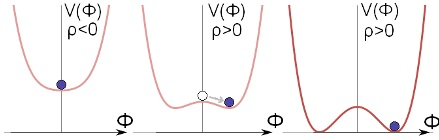
\includegraphics[width=0.4\textwidth]{./Figure/fig7_1.jpg}
	\figcaption{Higgs 势取不同参数$\rho$值的图像,$\rho$被认为是由于宇宙暴涨所造成的宇宙冷却而改变。Figure adapted from ``Spontaneous symmetry breaking'' by FT2 (Wikimedia Commons) released under a CC BY-SA 3.0 licence: \url{http://creativecommons.org/licenses/by-sa/3.0/deed.en}. URL:\url{http://commons.wikimedia.org/wiki/File:Spontaneous_symmetry_breaking_(explanatory_diagram).png}, Accessed: 8.12.2014}
	\label{fig:7.1}
}

这个想法是这样的:在相当高的温度下,例如宇宙早期,势能会像图左那样。极小值点,这里成为真空值,毫无疑问的在$\phi=0$处。参数$\lambda$和$\rho$随着温度的下降发生改变,势能的形状也是一样。当温度低于某个临界值时,如图右所示,$\phi=0$处不再是极小点。此时将会有许多点都能取到极小值。

事实上,这个势能有无穷多个极小值点。其可用通常的办法计算得到
\begin{align}
\label{equ7.70}
&V(\phi) = -\rho^2|\phi|^2 + \lambda |\phi|^4 \\
\label{equ7.71}
&\frac{\partial V(\phi)}{\partial \phi} = -2\rho^2|\phi|+4\lambda|\phi|^3 \\
\label{equ7.72}
\rightarrow &|\phi|(-2\rho^2+4\lambda|\phi|^2) \overset{\text{!}}{=} 0\\
\label{equ7.73}
\rightarrow &|\phi|^2  \overset{\text{!}}{=} \frac{\rho^2}{2\lambda} \\
\label{equ7.74}
\rightarrow &|\phi|  \overset{\text{!}}{=} \sqrt{\frac{\rho^2}{2\lambda}} \\
\label{equ7.75}
&\phi_{\min} = \sqrt{\frac{\rho^2}{2\lambda}} \ue^{\ri {\varphi}}\text{。}
\end{align}
这对于$\varphi$的任意取值都是极小值,所以我们有无穷多个极小点。全体极小点躺在了半径为$\sqrt{\frac{\rho^2}{2\lambda}}$的一个圆上。图\ref{fig:7.2}即为 Higgs 的三维图。就如同一粒弹珠从墨西哥草帽顶端自发而随机的滚落,一个新的真空值有无穷多种选择。
\marginpar{
	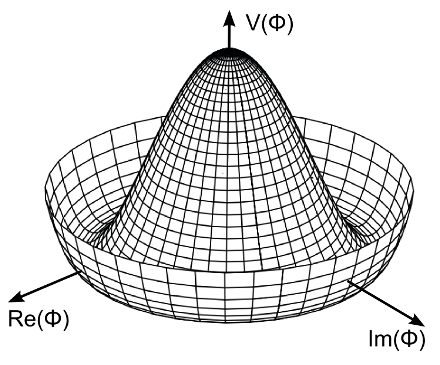
\includegraphics[width=0.4\textwidth]{Figure/fig7_2.png}
	\figcaption{Higgs 的三维图。 Figure adapted from ``Mexican hat potential polar'' by Rupert Millard (Wikimedia Commons) released under a public domain licence. URL:\url{http://commons.wikimedia.org/wiki/File:Mexican_hat_potential_polar.svg}, Accessed: 7.5.2014}
	\label{fig:7.2}
}

从\ref{equ7.69}中我们可知对于二重态,两个分量都需要作出这种选择。则对于二重态其极小点为
\begin{equation}
\label{equ7.76}
\Phi_{\min} = \begin{pmatrix}
\phi_{1\min} \\ \phi_{2\min}
\end{pmatrix}
\end{equation}
一个经济的{\bf 选择}%
\mpar{复习:对称破缺意味着{\bf 一个}极小值有无穷多种选取方式}%
是
\begin{equation}
\label{equ7.77}
\Phi_{\min} = \begin{pmatrix}
0 \\ \sqrt{\frac{\rho^2}{2\lambda}}
\end{pmatrix} \equiv \begin{pmatrix}
0 \\ \frac{v}{\sqrt{2}}
\end{pmatrix} \text{,}
\end{equation}
其中因子$\frac{1}{2}$只是为了使计算简洁而引入,自然有$v\equiv\sqrt{\frac{\rho^2}{\lambda}}$。下一步中我们会将场$\Phi$在极小值附近展开以得到想要的物理。之后我们将会学到,由于得不到精确解,量子场论中的计算总是围绕着极小值点的一系列级数。为了得到有意义的结果,我们必须将场移动到新的极小点。故我们考虑
\begin{equation}
\label{equ7.78}
\Phi = \begin{pmatrix}
\phi_{1r}+\ri \phi_{1c} \\ \frac{v}{\sqrt{2}} + \phi_{2r} + \ri \phi_{2c}
\end{pmatrix}\text{。}
\end{equation}

改写作\mpar{等会就能看到这个形式有多有用了。}
\begin{equation}
\Phi = \ue^{\ri \theta_i \frac{\sigma_i}{2}} \begin{pmatrix}
0 \\ \frac{v+h}{\sqrt{2}}
\end{pmatrix}\text{,}
\label{equ7.79}
\end{equation}
这是由于考虑将指数函数展开成级数,代入泡利矩阵$\sigma_i$矩阵的具体形式,在一阶意义上
\begin{align}
	\ue^{\ri \theta_i \frac{\sigma_i}{2}}
			\begin{pmatrix}
				0 \\ \frac{v+h}{\sqrt{2}}
			\end{pmatrix}
		&\approx (1+\ri \theta_i \frac{\sigma_i}{2})
			\begin{pmatrix}
				0 \\ \frac{v+h}{\sqrt{2}}
			\end{pmatrix}
	\nonumber \\
	&= \big(1 + \ri \theta_1 \frac{\sigma_1}{2}+\ri \theta_2 \frac{\sigma_2}{2}+\ri \theta_3 \frac{\sigma_3}{2} \big)
			\begin{pmatrix}
				0 \\ \frac{v+h}{\sqrt{2}}
			\end{pmatrix}
	\nonumber \\
	&=
		\begin{pmatrix}
			1 + \ri\frac{1}{2}\theta_3 & \frac{1}{2}\theta_1 - \ri \frac{1}{2}\theta_2 \\
			\frac{1}{2}\theta_1 + \ri \frac{1}{2}\theta_2 & 1 - \ri\frac{1}{2}\theta_3
		\end{pmatrix}
		\begin{pmatrix}
			0 \\ \frac{v+h}{\sqrt{2}}
		\end{pmatrix}
	\nonumber \\
	& =
		\begin{pmatrix}
			(\frac{1}{2}\theta_1 - \ri \frac{1}{2}\theta_2)\frac{v+h}{\sqrt{2}} \\ (1 - \ri\frac{1}{2}\theta_3)\frac{v+h}{\sqrt{2}}
		\end{pmatrix}
	\nonumber \\
\label{equ7.80}
	\text{重新定义}\rightarrow & \equiv
		\begin{pmatrix}
			\phi_{1r}+\ri \phi_{1c} \\ \frac{v}{\sqrt{2}}\phi_{2r}+\ri \phi_{2c}
		\end{pmatrix}\text{。}
\end{align}

将零自旋复二重态写成这个形式,有助于利用局域\sutw (规范)对称性化简计算。为了得到物理结果,我们必须选取{\bf 一个}规范,而合适的选择会使生活更美好%
\mpar{不同的规范适用于不同的问题。而这里我们采用的叫做幺正规范,这对理解一个理论的物理内容也是有益的。}。

一个一般的局域\sutw 变换写作
\begin{equation}
\label{equ7.81}
\Phi \rightarrow \Phi' = \ue^{\ri b_i(x)\frac{\sigma_i}{2}}\Phi\text{,}
\end{equation}
通过选取合适的$b_i(x)$,我们可以消去\ref{equ7.79}式中的指数因子。在{\bf 幺正规范(unitary gauge)}下,复标量二重态为
\begin{equation}
\Phi_{un} = \begin{pmatrix}
0 \\ \frac{v+h}{\sqrt{2}}
\end{pmatrix}\text{。}
\label{equ7.82}
\end{equation}
这件事也可以这样理解:复标量二重态的四个分量和\sutw 规范的自由度恰好相等%
\mpar{注意,这仅在满足如下这些条件下时成立:有一个局域\sutw 理论,场$\theta=\theta(x)$理所应当的依赖于时空坐标。对于一个全局对称性,这些分量怎么也不能被规范掉,此时将其解释为无质量 boson,称为 Goldstein bosons。}%
。这样,这三个场分量便是非物理的%
\mpar{局域\sutw 对称在实验上不存在任何可观测的效应。这仅仅是我们方程的对称性,规范自由度从不在任何实验测量量中出现。否则我们将无法做出预言,因为我们将有无穷多个相同可能性的预言(它们由\sutw 变换相联系)。尽管这样,这个对称性也不是没用的,它能将我们导向拉格朗日量的正确形式。}%
,不可能被实验观测到。最后留下来的便是{\bf 一个}物理场$h$,称作 {\bf Higgs 场}。

接下来,我们希望看看拉格朗日量对称性破缺的具体含义。我们将\ref{equ7.66}\footnote{\textcolor{red}{译注:原文引用公式有误,已更正}}式给出的拉格朗日量重新写在这里,并调整一下记号
\begin{equation}
\label{equ7.83}
\begin{aligned}
{\mathscr L} &= \bigg( (\partial_\mu-\ri g'\frac{1}{2}\sigma_i(W_\mu)_i-\ri\frac{1}{2}gB_\mu)\Phi^\dag \bigg) \bigg( (\partial^\mu+\ri g' \sigma_i(W^\mu)_i+\ri\frac{1}{2}gB^\mu)\Phi \bigg)\\
 & -V(\Phi)
\end{aligned}
\end{equation}
现在将场$\Phi$用平移且取幺正规范的场,即\ref{equ7.82}式代入。我们对新出现的包含有真空值$v$的项尤其感兴趣。而其他项描述了 Higgs 场的自作用以及 Higgs 场与其他场的相互作用,我们不会再对其做出进一步的讨论。我们将极小值点$\Phi\rightarrow\Phi_{\min}= \begin{pmatrix}
0 \\\frac{v}{\sqrt{2}}
\end{pmatrix}$(即不计入$h$),代入得
\[
\begin{aligned}
& \bigg( (\partial_\mu-\ri g'\frac{1}{2}\sigma_i(W_\mu)_i-\ri\frac{1}{2}gB_\mu)\Phi^\dag_{\min} \bigg)  \bigg( (\partial^\mu+\ri g'\frac{1}{2}\sigma_i(W^\mu)_i+\ri\frac{1}{2}gB^\mu)\Phi_{\min} \bigg) \\
& = \left|(\partial^\mu+\ri g'\frac{1}{2}\sigma_i(W^\mu)_i+\ri\frac{1}{2}gB^\mu)\Phi_{\min}\right|^2 \\
& = \left|(\partial^\mu+\ri g'\frac{1}{2}\sigma_i(W^\mu)_i+\ri\frac{1}{2}gB^\mu)\frac{1}{\sqrt{2}}\begin{pmatrix}
0 \\ v
\end{pmatrix}\right|^2 \\
& = \frac{v^2}{8} \left|( g'\sigma_i(W^\mu)_i+gB^\mu)\begin{pmatrix} 0 \\ 1 \end{pmatrix}\right|^2
\end{aligned}
\]
现在将用$2\times 2$单位阵表出的$B_\mu$和 Pauli 矩阵的具体形式\mpar{$\sigma_iW_i= \begin{pmatrix}
W_3 & W_1-\ri W_2 \\ W_1+\ri W_2 & -W_3
\end{pmatrix}$}代入得
\begin{equation}
\begin{aligned}
& = \frac{v^2}{8} \left|\begin{pmatrix}
g'W_3^\mu+gB^\mu & g'W_1^\mu-\ri g'W_2^\mu \\ g'W_1^\mu+\ri g'W_2^\mu & -g'W_3^\mu+gB^\mu
\end{pmatrix}\begin{pmatrix} 0 \\ 1 \end{pmatrix}\right|^2 \\
& = \frac{v^2}{8} \left|\begin{pmatrix}
g'W_1^\mu-\ri g'W_2^\mu \\  -g'W_3^\mu+gB^\mu
\end{pmatrix}\right|^2 \\
& = \frac{v^2}{8} \bigg( (g')^2 \big((W_1^\mu)^2+ (W_2^\mu)^2 \big) +  (g'W_3^\mu-gB^\mu)^2 \bigg)
\end{aligned}
\label{equ7.84}
\end{equation}

用已有的场定义两个新的自旋为$1$的场:
\begin{align}
\label{equ7.85}
W_+^\mu &\equiv \frac{1}{\sqrt{2}}(W_1-\ri W_2) \\
\label{equ7.86}
W_-^\mu &\equiv \frac{1}{\sqrt{2}}(W_1+\ri W_2)
\end{align}
即$W_+^\mu$是$W_-^\mu$的复共轭。\ref{equ7.84}式中的第一项可以写作
\begin{equation}
\label{equ7.87}
(W_1^\mu)^2+ (W_2^\mu)^2 = 2 (W^+)_\mu(W^-)^\mu
\end{equation}
把前面的常数添上,有
\begin{equation}
\label{equ7.88}
\left(\underbrace{\frac{g'v}{2}}_{\equiv m_W}\right)(W^+)_\mu(W^-)^\mu
\end{equation}
这就像一个典型的“质量”项。

\ref{equ7.84}式中的第二项可以写作矩阵形式\footnote{\textcolor{red}{译注:原文下式有误,已更正。}}
\begin{equation}
(g'W_3^\mu-gB^\mu)^2 = \begin{pmatrix}
(W_3)^\mu & B^\mu
\end{pmatrix} \underbrace{\begin{pmatrix}
g'^2 & -gg' \\ -gg' & g^2
\end{pmatrix}}_{\equiv G} \begin{pmatrix}
(W_3)_\mu \\ B_\mu
\end{pmatrix}
\label{equ7.89}
\end{equation}
为了将其解释为质量项,我们需要将矩阵$G$对角化%
\mpar{马上就能看到一个对角矩阵会带给我们和其他质量项长得一模一样的项。这使我们能将其对应的场诠释成实验上能够观测到的物理场。我们当然也可以就用$W_3^\mu$和$B^\mu$干活,但是却难以找到其直接的物理意义。}%
。线性代数说我们需要先得到矩阵$G$的本征值$\lambda_1$,$\lambda_2$以及归一%
\mpar{长度为一,即$v\cdot v= 1$。}%
的本征向量$v_1$,$v_2$。简单的计算得到
\[
\begin{aligned}
&\lambda_1 = 0 &\rightarrow v_1 = \frac{1}{\sqrt{g^2+g'^2}} \begin{pmatrix}
g\\ g'
\end{pmatrix} \\
&\lambda_2 = g^2+g'^2 &\rightarrow v_2 = \frac{1}{\sqrt{g^2+g'^2}} \begin{pmatrix}
g'\\ -g
\end{pmatrix}
\end{aligned}
\]
用本征向量排成的矩阵$M$可以将$G$对角化,即$G_\text{diag}=M^{-1}GM$,其中
\begin{equation}
\label{equ7.90}
M = \frac{1}{\sqrt{g^2+g'^2}} \begin{pmatrix}
g & g'\\ g'&-g
\end{pmatrix}
\end{equation}
以及
\begin{equation}
\label{equ7.91}
G_\text{diag} = \begin{pmatrix}
\lambda_1 & 0 \\ 0 & \lambda_2
\end{pmatrix} = \begin{pmatrix}
0 & 0 \\ 0 & g^2+g'^2
\end{pmatrix}
\end{equation}
由于我们用的是归一的本征向量,故矩阵$M$是正交的($M^T = M^{-1}$):
\begin{equation}
\label{equ7.92}
\begin{aligned}
M^TM & = \frac{1}{\sqrt{g^2+g'^2}} \begin{pmatrix}
g & g'\\ g'&-g
\end{pmatrix} \frac{1}{\sqrt{g^2+g'^2}} \begin{pmatrix}
g & g'\\ g'&-g
\end{pmatrix} \\
& = \frac{1}{g^2+g'^2} \begin{pmatrix}
g^2+g'^2 & gg'-gg'\\ gg'-gg'&g^2+g'^2
\end{pmatrix} = \begin{pmatrix}
1 & 0\\ 0 & 1
\end{pmatrix}\text{。}
\end{aligned}
\end{equation}
由此在\ref{equ7.89}式中插入两个单位阵$1 = M^TM$:
\begin{equation}
\label{equ7.93}
\begin{aligned}
&\begin{pmatrix}
(W_3)^\mu & B^\mu
\end{pmatrix} \underbrace{MM^T}_{=1} G \underbrace{MM^T}_{=1} \begin{pmatrix}
(W_3)_\mu \\ B_\mu
\end{pmatrix} \\ =& \begin{pmatrix}
(W_3)^\mu & B^\mu
\end{pmatrix} M\underbrace{M^TGM}_{=G_\text{diag}}M^T \begin{pmatrix}
(W_3)_\mu \\ B_\mu
\end{pmatrix} \text{。}
\end{aligned}
\end{equation}
剩下的任务即是计算$M^T \begin{pmatrix}
W_3^\mu \\ B_\mu
\end{pmatrix}$,以得到两个新的,有对应质量项的场:
\begin{equation}
\label{equ7.94}
\begin{aligned}
M^T \begin{pmatrix}
W_3^\mu & B_\mu
\end{pmatrix} &= \frac{1}{\sqrt{g^2+g'^2}} \begin{pmatrix}
g & g'\\ g'&-g
\end{pmatrix} \begin{pmatrix}
W_3^\mu \\ B_\mu
\end{pmatrix} \\
& = \frac{1}{\sqrt{g^2+g'^2}} \begin{pmatrix}
gW_3^\mu + g'B^\mu \\ gW_3^\mu - g'B^\mu
\end{pmatrix} \equiv \begin{pmatrix}
A^\mu \\ Z_\mu
\end{pmatrix}
\end{aligned}
\end{equation}
由此将第二项改做\footnote{译注:从而我们再次得到了\ref{equ7.84}式中的第二项——作者你绕了这么大一个弯子累不累啊?}
\begin{equation}
\label{equ7.95}
\begin{aligned}
\begin{pmatrix}
 A_\mu & Z_\mu
 \end{pmatrix} G_\text{diag} \begin{pmatrix}
 A^\mu \\ Z_\mu
 \end{pmatrix} &= \begin{pmatrix}
 A^\mu & Z_\mu
 \end{pmatrix} \begin{pmatrix}
0 & 0 \\ 0 & g^2+g'^2
\end{pmatrix} \begin{pmatrix}
 A^\mu \\ Z_\mu
 \end{pmatrix} \\
& = (g^2 + g'^2)(Z^\mu)^2 + 0\cdot (A^\mu)^2\text{。}
\end{aligned}
\end{equation}

综上,我们从自旋为$1$的无质量场$W_i^\mu$和$B^\mu$的拉格朗日量出发
\begin{equation}
\label{equ7.96}
(\partial_\mu-\ri g'\frac{1}{2}\sigma_i(W_\mu)_i-\ri\frac{1}{2}gB_\mu)\Phi^\dag(\partial^\mu+\ri g'\frac{1}{2}\sigma_i(W^\mu)_i+\ri\frac{1}{2}gB^\mu)\Phi\text{。}
\end{equation}
通过自发对称性破缺,我们在拉格朗日量中得到了可以被解释成质量项的新项
\begin{equation}
\label{equ7.97}
\underbrace{\frac{1}{8}v^2g'^2}_{=\frac{1}{2}M_W^2}(W^+)_\mu(W^-)^\mu + \underbrace{\frac{1}{8}v^2(g^2+g'^2)}_{=\frac{1}{2}M_Z^2}Z_\mu^2+  \underbrace{ \frac{1}{8}v^2\cdot 0}_{\text{光子质量为0}} \cdot A^2_\mu
\end{equation}

我们能看到其中一个自旋为$1$的场$A_\mu$在对称性自发破缺后仍然是无质量的。这是电磁的光子场,现有的所有实验都表明光子是无质量的%
\mpar{注意,在这一节中,我略去了一些重要的概念:超荷和 Weinberg 角。Weiberg 角 $\theta_W$由$\cos(\theta_W)=\frac{g}{g^2+g'^2}$或$\sin(\theta_W)=\frac{g'}{g^2+g'^2}$来定义。通过它可以简化本节中的一些记号。超荷略复杂一些,感兴趣的读者可以参考量子场论的标准教材,部分推荐数目见第\ref{chap9}章末。}%
。注意对应于 Z-bosons 的$Z_\mu$和对应于光子的$A_\mu$是场$B_\mu$和$W_\mu^3$的正交组合。它们竟有一个同样的起源!

同样的推演可以用来在不破坏局域\sutw 对称性的情况下得到\spint 场的质量项,但在具体讨论这个之前,我们需要先谈谈自然界中一个有趣的事实:宇称破坏。

\section[宇称破坏]{Parity Violation\quad 宇称破坏}
\label{sec7.4}
大自然不遵守宇称对称性,即宇称破坏,是科学史上最为重大的发现之一。通俗地说,宇称破坏使一部分物理实验表现出与其镜像实验所不同的物理现象。吴健雄在“吴实验”中最早发现了宇称破坏现象。这是一个漂亮的实验,但它的具体实现与本节主题无关,因此我们将只关注实验结果。

“吴实验”发现,弱相互作用的媒介子($W^+, W^-, Z$玻色子)仅与左手粒子耦合。换句话说,只有左手粒子才会通过弱作用力相互作用,这一物理机制与宇称破坏的关系将在本节结尾处加以解释。所有在弱相互作用中产生的粒子都是“左手”的。中微子只参与弱相互作用,因此右手中微子可能根本不存在\mpar{我们很快会看到,有质量的左手粒子总会在传播过程中获得右手分量。实验表明中微子有质量,因此也应当包含右手分量。然而这一右手分量不参与任何已知相互作用。}。另一方面,所有其它粒子都能通过另外三种相互作用产生,因此都可以具有“右手性”。

目前为止,我们用“左手性”和“右手性”,标注了对象在经历洛伦兹变换时所依据的群表示。这是一个抽象的概念,但我们却可以实际测量粒子的手性,因为抽象的“手性”概念直接关联于直观的“螺度”概念\mpar{此处我们不讨论这一概念,因其细节与本节叙述的主题无关。读者只需知道类似实验具有可行性。更多精彩的讨论可以参见以下文献:Alessandro Bettini. \textit{Introduction to Elementary Particle Physics}. Cambridge University Press, 2nd edition, 4 2014. ISBN 9781107050402}。

其实在多数情况下,微观粒子并没有确定的手性,也不处于确定的左手或右手态,而是由同时包含两种手性分量的狄拉克旋量所描述。宇称破坏并不是理论预言,相反,它的发现震惊了整个物理学界。即使到了今天,大自然这一奇特的性质依旧令人费解。然而,将这一发现纳入我们的理论框架却并不困难。我们只需利用某些数学工具,确保处理弱相互作用时只考虑左手旋量即可。

我们用$\chi, \xi$表示二分量外尔旋量,而$\psi$代表四分量狄拉克旋量:
\begin{align}
\psi=\begin{pmatrix}\chi_L\\\xi_R\end{pmatrix}
\label{equ7.98}
\end{align}
$\Psi$是狄拉克旋量的双重态:
\begin{align}
\Psi=\begin{pmatrix}\psi_1\\\psi_2\end{pmatrix}
\label{equ7.99}
\end{align}
上面提到的“某些工具”,是投影算符$P_L$:
\begin{align}
P_L\psi=P_L\begin{pmatrix}\chi_L\\\xi_R\end{pmatrix}=\begin{pmatrix}\chi_L\\0\end{pmatrix}\equiv \psi_L
\label{equ7.100}
\end{align}
投影算符可以用如下矩阵构造\mpar{请回忆方程\ref{equ6.13}中$\gamma_\mu$矩阵的定义,切记并无$\gamma_4$矩阵存在。由于另有规范以$\gamma_4$表示$\gamma_0$。为避免符号混淆,此处特将这一矩阵记为$\gamma_5$。}:
\begin{align}
\gamma_5=i\gamma_0\gamma_1\gamma_2\gamma_3=\begin{pmatrix}-1 & 0 \\ 0 & 1\end{pmatrix}
\label{equ7.101}
\end{align}
矩阵$\gamma_5$被称为{\bf 手性算符},因为单一手性态$\begin{pmatrix}\chi_L\\0\end{pmatrix}$或$\begin{pmatrix}0\\\xi_R\end{pmatrix}$,正是$\gamma_5$本征值为$-1$和$+1$的两个本征态。

于是,投影算符$P_L$可以写为\mpar{读者可能会问,为什么我们要用这样复杂的方式定义$P_L$,而不是直接从矩阵形式出发呢?这样做的目的,是为了保留在其它基下工作的可能性,那时$\gamma_\mu$的矩阵形式可以非常不同。(读者可以在\ref{sec8.10}节中找到更多信息)注意到拉氏量中狄拉克旋量总与$\gamma_\mu$相伴出现。在这两者之间,我们总可以插入$1=\mathcal{U}^{-1}\mathcal{U}$,其中$\mathcal{U}$为任意可逆矩阵。例如$\partial_\mu\bar{\Psi}\gamma_\mu\Psi=\partial_\mu\bar{\Psi}\underbrace{\mathcal{U}^{-1}\mathcal{U}}_{=1}\gamma_\mu\underbrace{\mathcal{U}^{-1}\mathcal{U}}_{=1}\Psi=\partial_\mu\underbrace{\bar{\Psi}\mathcal{U}^{-1}}_{=\bar{\Psi}'}\underbrace{\mathcal{U}\gamma_\mu\mathcal{U}^{-1}}_{\gamma_\mu'}\underbrace{\mathcal{U}\Psi}_{\Psi'}$。物理事实当然独立于这类基矢变换,我们却可以利用它简化计算。本书正文偏好使用的基矢,被称为 Weyl 基。在其它基矢下,狄拉克旋量的两个分量是$\chi_L$与$\xi_R$的混合。尽管如此,通过$P_L=\frac{1-\gamma_5}{2}$定义的投影算符,总能将其投影为左手分量。这是因为$P^\text{Weyl}_L\Psi^\text{Weyl}=\Psi^\text{Weyl}_L\Rightarrow P_L'\Psi'=\frac{1-\gamma_5'}{2}\ \underbrace{\Psi'}_{\mathcal{U}\Psi^\text{Weyl}}=\frac{1-\mathcal{U}i\gamma_0\mathcal{U}^{-1}\mathcal{U}\gamma_1\mathcal{U}^{-1}\mathcal{U}\gamma_2\mathcal{U}^{-1}\mathcal{U}\gamma_3\mathcal{U}^{-1}}{2}\ \mathcal{U}\Psi^\text{Weyl}=\frac{\mathcal{U}-\mathcal{U}i\gamma_0\gamma_1\gamma_2\gamma_3}{2}\Psi^\text{Weyl}=\mathcal{U}\left(\frac{1-\gamma_5}{2}\right)\Psi^\text{Weyl}=\mathcal{U}\Psi^\text{Weyl}_L=\Psi_L'\quad\checkmark$}
\begin{align}
P_L=\frac{1-\gamma_5}{2}=\begin{pmatrix}1 & 0 \\ 0 & 0\end{pmatrix}
\label{equ7.102}
\end{align}
类似的,我们定义
\begin{align}
P_R=\frac{1+\gamma_5}{2}=\begin{pmatrix}0 & 0 \\ 0 & 1\end{pmatrix}
\label{equ7.103}
\end{align}
现在为了限制只有左手粒子参与弱相互作用,我们必须在拉氏量中,描述各类场与$W^\pm_\mu$与$Z_\mu$相互作用的每一项里都插入$P_L$。这些项已在\ref{sec7.2}节中导出,最终结果参看方程\ref{equ7.58},我们将其重写如下:
\begin{align}
\mathscr{L}=i\bar{\Psi}\gamma_\mu\partial^\mu\Psi+i\bar{\Psi}\gamma_\mu\sigma_j W_j^\mu \Psi-\frac{1}{4}(W_{\mu\nu})_i(W^{\mu\nu})_i
\label{equ7.104}
\end{align}
其中需要处理的一项是$\bar{\Psi}\gamma_\mu\sigma_j W^\mu_j\Psi$,我们将$P_L$插入:
\begin{align}
\rightarrow\mathscr{L}=i\bar{\Psi}\gamma_\mu\partial^\mu\Psi+i\bar{\Psi}\gamma_\mu\sigma_j W_j^\mu P_L\Psi-\frac{1}{4}(W_{\mu\nu})_i(W^{\mu\nu})_i
\label{equ7.105}
\end{align}
此处$P_L$作用于双重态,得到
\begin{align}
P_L\Psi=\begin{pmatrix}P_L & 0 \\ 0 & P_L\end{pmatrix}\begin{pmatrix}\psi_1\\\psi_2\end{pmatrix}=\begin{pmatrix}(\psi_1)_L\\(\psi_2)_L\end{pmatrix}
\label{equ7.106}
\end{align}

我们断言,只需在表达式中插入一个$P_L$, 就可以将$\bar{\Psi}$和$\Psi$同时投影到左手分量上。为了理解这一点,我们需要以下三个等式:
\begin{itemize}
\item $(P_L)^2 = P_L$,这可以从算符的矩阵形式立即看出,同时也是投影算符必须满足的性质\mpar{投影算符的定义中还包括$P_LP_R=P_RP_L=0$,此处可用$P_L,P_R$和$\gamma_5$的矩阵形式验证成立。}。两次投影应等价于一次投影。
\item $\{\gamma_5,\gamma_\mu\}=\gamma_5\gamma_\mu+\gamma_\mu\gamma_5=0$,这可以通过简单粗暴的展开计算加以证明\mpar{或可用定义$\gamma_5=i\gamma_0\gamma_1\gamma_2\gamma_3$结合以下等式证明:$\{\gamma_\mu,\gamma_\nu\}=\gamma_\mu\gamma_\nu+\gamma_\nu\gamma_\mu=\frac{1}{2}\eta_{\mu\nu}$,其中$\eta_{\mu\nu}$为 Minkowski 度规。}。
\item $(P_L)^\dag=P_L$,因为$\gamma_5$是实矩阵。而这一点可以从$\gamma_5$的矩阵形式直接看出$\gamma_5=\begin{pmatrix}-1 & 0 \\ 0 & 1\end{pmatrix}$。

\end{itemize}

第二个等式直接推出$\gamma_5\gamma_\mu=-\gamma_\mu\gamma_5$,即我们可以交换$\gamma_5$和$\gamma_\mu$矩阵的位置,只需加入一个额外的负号。于是我们有:
\begin{align}
\gamma_\mu P_L=\gamma_\mu\frac{1-\gamma_5}{2}=\frac{1+\gamma_5}{2}\gamma_\mu=P_R\gamma_\mu
\label{equ7.107}
\end{align}

现在我们可以将方程\ref{equ7.105}中的相关项写为:
\begin{align}
\bar{\Psi}\gamma_\mu\sigma_j W_j^\mu P_L\Psi&=\bar{\Psi}\gamma_\mu\sigma_j W_j^\mu (P_L)^2\Psi\nonumber\\
&=\underbrace{\bar{\Psi}}_{\Psi^\dag\gamma_0}\underbrace{\gamma_\mu P_L}_{P_R\gamma_\mu}\sigma_j W_j^\mu \underbrace{P_L\Psi}_{\Psi_L}\nonumber\\
&=\Psi^\dag\underbrace{\gamma_0P_R}_{P_L\gamma_0}\gamma_\mu\sigma_j W_j^\mu \Psi_L\nonumber\\
&\underbrace{=}_{\mathclap{\text{利用}P_L^\dag=P_L\text{以及}(AB)^\dag=((AB)^T)^*=(B^TA^T)^*=B^\dag A^\dag}}(P_L\Psi)^\dag\gamma_0\gamma_\mu\sigma_j W_j^\mu \Psi_L\nonumber\\
&=(\underbrace{P_L\Psi}_{=\Psi_L})^\dag\gamma_0\gamma_\mu\sigma_j W_j^\mu \Psi_L\nonumber\\
&=\bar{\Psi}_L\gamma_\mu\sigma_j W_j^\mu \Psi_L\text{\hspace{7mm}\checkmark}
\label{equ7.108}
\end{align}
{\bf 至此,我们已经知道了,如何在数学上描述只有左手粒子参与弱相互作用的物理事实。然而,为什么这就意味着宇称破坏?}为了理解这一点,我们需要对相互作用项进行宇称变换。因为在宇称变换下这一项不具有不变性,由这一项描述的物理系统,也将和它的“镜像”有所不同\mpar{这就是说,若一项实验的结果全由拉氏量中的这一项所决定,那么当实验设置全部以镜像方式反转时,实验结果也会有所不同。}。这里我们用到旋量\mpar{旋量宇称算符在\ref{sec3.7.9}节中导出。用$\gamma_\mu$矩阵,我们可以将宇称算符写作$P=\gamma_0=\begin{pmatrix}0 & \sigma_0\\ \sigma_0 & 0\end{pmatrix}=\begin{pmatrix}0 & 1 \\ 1 & 0\end{pmatrix}$}和矢量\mpar{矢量宇称算符即为$P_\text{vector}=\begin{pmatrix}1 & 0 & 0 & 0 \\  0 & -1 & 0 & 0 \\ 0 & 0 & -1 & 0 \\ 0 & 0 & 0 & -1 \\ \end{pmatrix}$,如方程\ref{equ3.132}所述。}的宇称算符$P_\text{spinor}$, $P_\text{vector}$。在宇称变换下:
\begin{align}
\underbrace{\bar{\Psi}}_{=\Psi^\dag\gamma_0}\gamma_\mu\sigma_j (W_j^\mu) P_L\Psi\rightarrow(P_\text{spinor}&\Psi)^\dag\gamma_0\gamma_\mu\sigma_j (P_\text{vector}W^\mu)_j P_L(P_\text{spinor}\Psi)\nonumber\\
&=(\Psi)^\dag\gamma_0\gamma_0\gamma_\mu\sigma_j (P_\text{vector}W^\mu)_j P_L\gamma_0\Psi\nonumber\\
&\underbrace{=}_{\mathclap{\text{利用}\{\gamma_5,\gamma_0\}=0\text{以及}P_L=\frac{1-\gamma_5}{2}}}(\Psi)^\dag\gamma_0\gamma_0\gamma_\mu\sigma_j (P_\text{vector}W^\mu)_j P_R\Psi.
\label{equ7.109}
\end{align}
我们可以通过矩阵运算得到$\gamma_0\gamma_0\gamma_0=\gamma_0$及$\gamma_0\gamma_i\gamma_0=-\gamma_i$。同时,我们通过$P_\text{vector}$的表达式看出$P_\text{vector}W^0 = W^0$及$P_\text{vector}W^i = -W^i$。此处两负号相互抵消,于是拉氏量中的这一项,在宇称变换下变为
\begin{align}
(P_\text{spinor}\Psi)^\dag\gamma_0\gamma_\mu(P_\text{vector}W^\mu)_jP_L(P_\text{spinor}\Psi)=\bar{\Psi}\gamma_\mu\sigma_j W_j^\mu P_R\Psi\ne\bar{\Psi}\gamma_\mu\sigma_j W_j^\mu P_L\Psi
\label{equ7.110}
\end{align}

\textbf{因此这一项不具有不变性,也就违反了宇称对称性。}

宇称破坏还有一个重要的推论。还记得,我们会把那些在变换下相互转变的东西%
\mpar{详见附录 A 中的解释。}%
竖着放在一起,夹在两个括号之间。比如我们讨论四维矢量,是因为它的分量在空间转动和推动下可以相互转化。在这一节中,我们知道只有左手粒子参与弱相互作用,而描述这一现象的正确拉氏量写作$\bar{\Psi}\gamma_\mu\sigma_j W_j^\mu P_L\Psi=\bar{\Psi}_L\gamma_\mu\sigma_j W_j^\mu\Psi_L$。从物理上说,这一项表明组成左手旋量双重态的两个分量,即两个自旋$1/2$场$(\psi_1)_L,(\psi_2)_L$可以通过弱作用相互转化。而右手场不参与弱相互作用,因而$(\psi_1)_R,(\psi_2)_R$无法相互转化。可见,我们没有理由将两个右手分量写成双重态的形式。在数学上,这意味着右手场构成$\mathcal{SU}(2)${\bf 单态},也就是说,它们在对称操作下将根据$\mathcal{SU}(2)$群的一维表示变换。从\ref{sec3.6.3}节的讨论中我们知道,这等于说右手场实际上在变换下不变。最后我们加以总结:
\begin{itemize}
\item 左手场构成$\mathcal{SU}(2)${\bf 双重态}:$\Psi_L=\begin{pmatrix}(\psi_1)_L\\ (\psi_2)_L\end{pmatrix}$,因为它们都参与弱相互作用,可以互相转化。它们根据$\mathcal{SU}(2)$群的二维表示变换:
\begin{align}
\Psi_L\rightarrow\Psi'_L=e^{i\vec{a}\frac{\vec{\sigma}}{2}}\Psi_L
\label{equ7.111}
\end{align}
\item 右手场由$\mathcal{SU}(2)$单态描述:$(\psi_1)_R$,$(\psi_2)_R$,因为它们不参与弱相互作用,因而不能相互转化。它们根据$\mathcal{SU}(2)$的一维表示变换:
\begin{align}
&(\psi_1)_R\rightarrow (\psi_1)'_R=\mathrm{e}^0(\psi_1)_R=(\psi_1)_R\nonumber\\
&(\psi_2)_R\rightarrow (\psi_2)'_R=\mathrm{e}^0(\psi_2)_R=(\psi_2)_R
\label{equ7.112}
\end{align}
\end{itemize}

下面我们将继续讨论如何在保持原有对称性的前提下,于拉氏量中加入自旋$\frac{1}{2}$粒子的质量项。


\section[轻子质量项]{Lepton Mass Terms\quad 轻子质量项}\label{sec7.5}

在\ref{sec7.2}节开头,我们发现无法既保证$\mathcal{SU}(2)$对称性,又在拉氏量中加入任意的质量项$\bar{\Psi}m\Psi$。在这一节里,我们会看到宇称破坏让问题变得更加复杂。最后我们将再次引入希格斯机制解决这一难题。

在上一节中,我们讨论了耦合项$\bar{\Psi}\gamma_\mu\sigma_jW_j^\mu P_L\Psi$的手性。然而质量项的手性又如何呢?回顾我们在方程\ref{equ6.7}与\ref{equ6.8}中导出的,不含导数的旋量不变量:
\begin{align}
I_1:=(\chi_a)^\dag\xi^{\dot a}=(\chi_L)^\dag\xi_R\quad\text{和 }I_2:=(\xi^a)^T\chi_a=(\xi_R)^\dag\chi_L
\label{equ7.113}
\end{align}

我们可以用狄拉克旋量将其写为\mpar{如上节所述,狄拉克旋量$\psi_L$和$\psi_R$由手性投影算符定义:$\psi_L=P_L\psi$和$\psi_R=P_R\psi$。注意$\bar{\psi}=\psi^\dag\gamma_0$}:
\begin{align}
\bar{\psi}\psi&=\bar{\psi}_L\psi_R+\bar{\psi}_R\psi_L\nonumber\\
&=\begin{pmatrix}\chi_L^\dag & 0\end{pmatrix}\begin{pmatrix}0 & \sigma_0 \\ \sigma_0 & 0\end{pmatrix}\begin{pmatrix}0 \\ \xi_R\end{pmatrix}\nonumber\\
&=\chi_L^\dag\xi_R+\xi_R^\dag\chi_L\quad\checkmark
\label{equ7.114}
\end{align}

我们看到,洛伦兹不变的质量项包含左手与右手场的乘积。上节结尾处提到,左手场与右手场在$\mathcal{SU}(2)$变换下有不同的变换性质,这就产生了问题。左手场是双重态,而右手场是单态。双重态和单态的乘积不再是$\mathcal{SU}(2)$不变量。如:
\begin{align}
\underbrace{\bar{\Psi}}_\text{双重态}\underbrace{\psi_R}_\text{单态}\rightarrow \bar{\Psi}'_L\psi'_R=\bar{\Psi}_Le^{-ib_i\frac{\sigma_i}{2}}\psi_R\ne \bar{\Psi}_L\psi_R
\label{equ7.115}
\end{align}

基于处理自旋1场质量项的经验,我们重规叠矩,不加入上述质量项,而是在拉氏量中加入与0自旋场耦合,且满足$\mathcal{SU}(2)$不变的相互作用项。此后通过选择0自旋场的真空期望值,破缺这一对称性,进而制造出质量项。

耦合0自旋双重态与自旋$\frac{1}{2}$场,且保证$\mathcal{SU}(2),\mathcal{U}(1)$与洛伦兹不变性的项,由下式给出:
\begin{align}
\bar{\Psi}_L\Phi\psi_R
\label{7.116}
\end{align}

为验证其不变性,我们将$\mathcal{SU}(2)$变换作用于上式\mpar{注意到$\Phi^L\rightarrow\Phi'^{L}=e^{ib_i(x)\sigma_i}\Phi^L$,及$\sigma_i^\dag=\sigma_i$。}
\begin{align*}
\bar{\Psi}^L\Phi\psi^R\rightarrow\bar{\Psi}'^{L}\Phi\psi'^R=\bar{\Psi}^Le^{-ib_i(x)\sigma_i}\Phi e^{ib_i(x)\sigma_i}\psi^R=\bar{\Psi}^L\Phi\psi^R\quad\checkmark
\end{align*}
同时作用$\mathcal{U}(1)$变换
\begin{align*}
\bar{\Psi}^L\Phi\psi^R\rightarrow\bar{\Psi}'^{L}\Phi\psi'^R=\bar{\Psi}^Le^{-ia(x)}\Phi e^{ia(x)}\psi^R=\bar{\Psi}^L\Phi\psi^R\quad\checkmark
\end{align*}

0自旋场(洛伦兹标量)在洛伦兹变换下不变\mpar{0自旋场根据定义,应随洛伦兹群的$(0,0)$表示变换。在这一表示中,所有洛伦兹变换都是恒等变换。在\ref{sec3.7.4}中我们导出了这一结论。},于是这一项为洛伦兹不变量,因为它的其余因子与方程\ref{equ7.114}相同。

这类相互作用项被称为{\bf Yukawa耦合}。我们将这一项与其厄米共轭结合,再乘以耦合常数\mpar{稍后,我们会讨论包含$\psi_1^R$和$-\lambda_1$的相互作用项。届时,读者就能明白为什么我们将耦合常数记为$-\lambda_2$,以及下式为何只包含$\psi_2^R$。}$-\lambda_2$,加入到拉氏量之中。
\begin{align}
\mathscr{L}=-\lambda_2(\bar{\Psi}^L\Phi\psi_2^R+\bar{\psi}^R_2\Phi\Psi^L)
\label{7.117}
\end{align}

这一额外项不仅描述了fermion与Higgs场的耦合,也在$\mathcal{SU}(2)$对称性破缺后导致了fermion质量项的产生。我们在真空期望附近展开,选择方程\ref{equ7.77}
\begin{align*}
\Phi=\sqrt{\frac{1}{2}}\begin{pmatrix}0 \\ v+h\end{pmatrix}
\end{align*}

将其代入拉氏量,得到
\begin{align*}
\mathscr{L}&=-\frac{\lambda_2}{\sqrt{2}}\left(\begin{pmatrix}\bar{\Psi}_1^L,\bar{\Psi}^L_2\end{pmatrix}\begin{pmatrix}0 \\ v+h\end{pmatrix}\psi^R_2+\bar{\psi}^R_2\begin{pmatrix}0,v+h\end{pmatrix}\begin{pmatrix}\Psi^L_1 \\ \Psi^L_2\end{pmatrix}\right)\nonumber\\
&=-\frac{\lambda_2(v+h)}{\sqrt{2}}(\bar{\Psi}_2^L\psi_2^R+\bar{\psi}^R_2\Psi^L_2)
\end{align*}

由方程\ref{equ7.114}可知上式等价于
\begin{align}
=-\frac{\lambda_2(v+h)}{\sqrt{2}}\bar{\psi}_2\psi_2
\label{equ7.118}
\end{align}
\begin{align}
=\underbrace{-\frac{\lambda_2v}{\sqrt{2}}\bar{\psi}_2\psi_2}_\text{Fermion质量项}-\underbrace{\frac{\lambda_fh}{\sqrt{2}}\bar{\psi}_2\psi_2}_\text{Fermion-Higgs相互作用}
\label{equ7.119}
\end{align}

可见,Higgs机制确实导致了质量项的产生。再一次,我们根据对称性约束为拉氏量添加Higgs耦合项,并在对称破缺后产生出自旋$\frac{1}{2}$场的质量项。值得注意的是,只有双重态中的第二个场$\psi_2$获得了质量项。那么第一个场$\psi_1$怎么办呢?

为了获得$\Psi_1$的质量项,我们考虑电荷共轭\mpar{\ref{sec3.7.10}节探讨了电荷共轭的概念。}Higgs场$\tilde{\Psi}=\epsilon\Psi^*$的耦合项。由于
\begin{align}
\Phi=\begin{pmatrix}0 \\ \frac{v+h}{\sqrt{2}}\end{pmatrix}\rightarrow\tilde{\Phi}=\epsilon\Phi^*=\begin{pmatrix}0 & 1 \\ -1 & 0\end{pmatrix}\begin{pmatrix}0 \\ \frac{v+h}{\sqrt{2}}\end{pmatrix}=\begin{pmatrix} \frac{v+h}{\sqrt{2}} \\ 0\end{pmatrix}
\label{equ7.120}
\end{align}

对电荷共轭Higgs场重复上面的推导步骤,即可获得$\Psi_1$的质量项
\begin{gather*}
\mathscr{L}=-\lambda_f(\bar{\Psi}^L\tilde{\Phi}\psi_1^R+\bar{\psi}^R_1\tilde{\Phi}\Psi^l)\nonumber\\
=-\frac{\lambda_1}{\sqrt{2}}\left(\begin{pmatrix}\bar{\Psi}_1^L,\bar{\Psi}_2^L\end{pmatrix}\begin{pmatrix}\frac{v+h}{\sqrt{2}}\\0\end{pmatrix}\Psi_1^R+\bar{\Psi}_1^R\begin{pmatrix}\frac{v+h}{\sqrt{2}} \\ 0\end{pmatrix}\begin{pmatrix}\Psi^L_1 \\ \Psi^L_2\end{pmatrix}\right)\\
=-\frac{\lambda_1(v+h)}{\sqrt{2}}\left(\bar{\Psi}_1^L\Psi_1^R+\bar{\Psi}_1^R\Psi_1^L  \right)
\end{gather*}


为更好地理解这一抽象的双重态,我们将其重写如下\mpar{$\nu$永远代表中微子。在此处,我们给出双重态$\psi_1$和$\psi_2$中两分量的传统命名:电子场$e$和电子中微子场$\nu_e$。}:
\begin{align}
\Psi=\begin{pmatrix}\nu_e \\ e\end{pmatrix}
\label{7.121}
\end{align}
其它轻子,即$\mu,\nu_\mu$与$\tau,\nu_\tau$也有等价的写法。这一写法是由实验结果所确定的,因为在弱相互作用下,电子要么转化为动量可能不同的另一电子,要么变为电子中微子$\nu_e$与其它粒子的集合。在弱相互作用中,$e$和$\nu_e$(同样包括$\mu,\nu_\mu$与$\tau,\nu_\tau$)总是相伴出现。这一事实可以用耦合项$\bar{\Psi}\gamma_\mu\sigma_jW_j^\mu P_L\Psi$的数学形式加以解释。如前一节所述,这一项可以用Pauli矩阵$\sigma_i$的矩阵形式加以重写\mpar{这再次给出$\sigma_i W_i^\mu=\begin{pmatrix}W_3^\mu & W_1^\mu-iW_2^\mu \\ W_1^\mu+iW_2^\mu & -W_3^\mu\end{pmatrix}$。这可以用下式进行简化:$W_{\pm}=\frac{1}{\sqrt{2}}(W_1\pm W_2)\Rightarrow \sigma_i W_i^\mu=\begin{pmatrix}W_3^\mu & \sqrt{2}W_+ \\ \sqrt{2}W_- & -W_3^\mu\end{pmatrix}$},并给出双重态两分量间的耦合项。
\begin{align}
\bar{\Psi}\gamma_\mu\sigma_jW_j^\mu P_L\Psi&=\begin{pmatrix}\bar{\nu}_e & \bar{e}\end{pmatrix}\gamma_\mu \begin{pmatrix}W_3^\mu & \sqrt{2}W_+ \\ \sqrt{2}W_- & -W^\mu_3\end{pmatrix}P_L\begin{pmatrix}\nu_e \\ e\end{pmatrix}\nonumber\\
&\underbrace{=}_{\mathclap{\text{使用方程\ref{equ7.105}}}}\begin{pmatrix}(\bar{\nu}_e)_L & (\bar{e})_L\end{pmatrix}\gamma_\mu \begin{pmatrix}W_3^\mu & \sqrt{2}W_+ \\ \sqrt{2}W_- & -W^\mu_3\end{pmatrix}P_L\begin{pmatrix}(\nu_e)_L \\ (e)_L\end{pmatrix}\nonumber\\
&=(\bar{\nu}_e)_L\gamma_\mu W^\mu_3(\nu_e)_L+(\bar{\nu}_e)_L\gamma_\mu\sqrt{2}W_+(e)_L\nonumber\\&\quad+(\bar{e})_L\gamma_\mu\sqrt{2}W_-(\nu_e)_L-(\bar{e})_L\gamma_\mu W^\mu_3(e)_L
\label{7.122}
\end{align}
如果我们想同时考虑包括$e,\mu,\tau$的所有轻子产生过程,需将相应的三个耦合项都写入拉氏量:
\begin{align}
\bar{\Psi}_e\gamma_\mu\sigma_jW_j^\mu P_L\Psi_e+\bar{\Psi}_\mu\gamma_\mu\sigma_jW_j^\mu P_L\Psi_\mu+\bar{\Psi}_\tau\gamma_\mu\sigma_jW_j^\mu P_L\Psi_\tau
\label{7.123}
\end{align}

引入$\Psi_l=\begin{pmatrix} \nu_l \\ l \end{pmatrix}$,其中$l=e,\mu,\tau$,上式可写为更紧凑的形式:
\begin{align*}
\bar{\Psi}_L\gamma_\mu\sigma_jW_j^\mu P_L\Psi_L
\end{align*}

定义$l=\begin{pmatrix} l_L \\ l_R \end{pmatrix}$,质量项可写为:
\begin{align*}
\underbrace{-\frac{\lambda_lv}{\sqrt{2}}(\bar{l}{l})}_{\text{Fermion 质量项}} -\qquad \underbrace{\frac{\lambda_fh}{\sqrt{2}}(\bar{l}{l})}_{\mathclap{\text{Fermion-Higgs 相互作用}}}
\end{align*}

对中微子也有等价的形式。

这一拉氏量可以用来预测有关Higgs场的实验现象。轻子质量由下式给出:
\begin{align}
m_l=\frac{\lambda_lv}{\sqrt{2}}\rightarrow \lambda_l=\frac{m_l\sqrt{2}}{v}
\label{equ7.124}
\end{align}
而轻子与Higgs场的耦合强度为:

\begin{align}
c_l=\frac{\lambda_lh}{\sqrt{2}}\underbrace{=}_{\text{方程\ref{equ7.124}}}\frac{m_l\sqrt{2}h}{\sqrt{2}v}=\frac{m_lh}{v}
\label{equ7.125}
\end{align}

从这一方程可以看出,Higgs场与给定轻子的耦合强度,正比于这一轻子的质量。轻子质量越大,耦合强度越强。运用类似的推导,我们可将这一结论推广到所有粒子。

参与弱相互作用的自旋$\frac{1}{2}$粒子还包括{\bf 夸克}。同时,夸克还参与第三种相互作用:强相互作用。这一内容将在\ref{sec7.8}节中讨论。首先我们将讨论夸克的质量项,可喜的是,这一主题可用类似引入轻子质量的方法加以处理。

\section[夸克质量项]{Quark Mass Terms\quad 夸克质量项}\label{sec7.6}
在上一节中我们知道,$\mathcal{SU}(2)$双重态包含了两种可通过弱作用力相互转化的粒子。就夸克\mpar{没听说过夸克?请看\ref{sec1.3}节。}而言,这两种粒子是上夸克和下夸克。
\begin{align}
q=\begin{pmatrix}u\\d\end{pmatrix}
\label{equ7.126}
\end{align}
类似的,奇夸克、粲夸克,和顶夸克、底夸克也各自组成双重态。

与前文一样,考虑到只有左手粒子参与弱相互作用的实验事实,我们构造左手双重态和右手单态:
\begin{align}
\underbrace{q_L}_{\text{双重态}}=\begin{pmatrix}u_L\\d_L\end{pmatrix}\quad\rightarrow\quad e^{ia_i\frac{\sigma_i}{2}}q_L
\label{equ7.127}
\end{align}
\begin{align}
\underbrace{u_R}_{\text{单态}}\quad\rightarrow\quad u_R\nonumber\\
\underbrace{d_R}_{\text{单态}}\quad\rightarrow\quad d_R
\label{equ7.128}
\end{align}

右手粒子依旧不参与弱相互作用,不能转化为任何其它粒子,只构成$\mathcal{SU}(2)$单态(单分量的数学对象)。

这里,我们遇到了与处理轻子质量时相同的疑难:为了得到洛伦兹不变量,我们需要组合左、右手旋量。然而,这样的组合却不满足$\mathcal{SU}(2)$不变性,这让我们转而选择引入Higgs机制。换而言之,我们放弃在拉氏量中直接加入质量项:

\begin{align}
\bar{q}_Lu_R+\bar{q}_Ld_R+\bar{u}_Rq_L+\bar{d}_Rq_L
\label{equ7.129}
\end{align}

因为它不满足$\mathcal{SU}(2)$不变性。相反,我们考虑夸克与0自旋场$\Psi$的耦合项:
\begin{align}
\lambda_u\bar{q}_L\tilde{\Phi}u_R+\lambda_d\bar{q}_L\Phi d_R+\lambda_u\bar{u}_R\tilde{\Phi}q_L+\lambda_d\bar{d}_R{\Phi}q_L
\label{equ7.130}
\end{align}
这里我们引入耦合常数$\lambda_u,\lambda_d$和电荷共轭Higgs双重态\mpar{即方程\ref{equ7.120},$\tilde{\Phi}=\epsilon\Phi^*\underbrace{=}=\begin{pmatrix}\frac{v+h}{\sqrt{2}} \\ 0 \end{pmatrix}$},后者为上夸克提供了质量项\mpar{我们将双重态定义为$\begin{pmatrix}u \\ d \end{pmatrix}$。其与$\Phi=\begin{pmatrix}0 \\ \frac{v+h}{\sqrt{2}}  \end{pmatrix}$的乘积正比于$d$。}。

可见,这里的全部数学构造,都类比于处理轻子质量时所用的方法:我们在最小值附近展开Higgs场\mpar{$\Phi=\begin{pmatrix}0 \\ \frac{v+h}{\sqrt{2}}  \end{pmatrix}$,电荷共轭Higgs场有类似结论。},代入拉氏量,制造出质量项和夸克——Higgs耦合项。

\section[同位旋]{Isospin \quad 同位旋}\label{sec7.7}
现在讨论$\mathcal{SU}(2)$对称性所对应的守恒量。自由拉氏量只具有全局对称性,而加入相互作用项,则为其引入了局域对称性。注意到全局对称性是局域对称性的特例,因此全局对称性也存在于所有局域对称的拉氏量之中,其对应的守恒量也在两种情况下都守恒。由于Noether定理,$\mathcal{SU}(2)$对称性给出了一个新的守恒量:同位旋。同位旋与电荷类似,后者对应全局$\mathcal{U}(1)$对称性。

将Noether定理应用于内部对称性(见\ref{sec4.5.5}节,参考方程\ref{equ4.56})得到,
\begin{align}
\partial_0\int{d^3x\underbrace{\frac{\partial\mathscr{L}}{\partial(\partial_0\Psi)}\delta\Psi}_{=Q}}=0
\label{equ7.131}
\end{align}
拉氏量在下述形式的变换下不变:
\begin{align}
\Psi\rightarrow e^{ia_i\frac{\sigma_i}{2}}\Psi=(1+ia_i\frac{\sigma_i}{2}+\ldots)\Psi
\label{equ7.132}
\end{align}
于是无穷小变分写为$\delta\Psi=ia_i\frac{\sigma_i}{2}  \Psi$,其中$a_i$为任意系数。可见每个生成元都对应了一个守恒量,因为取$a_i$中任意两个为0、第三个不为0时,拉氏量同样具有不变性。比如$a_2=a_3=0$而$a_1\ne0$,或$a_1=a_2=0$而$a_3\ne0$。当然,取$a_1\ne0,a_2\ne0$且$a_3\ne0$时我们还能得到一个守恒量,但它其实是上述与生成元对应的三个守恒量之和。换而言之,一共有三个独立的守恒量,它们与$\mathcal{SU}(2)$生成元一一对应。

全局不变的自由拉氏量写为(方程\ref{equ7.45}):
\begin{align*}
\mathscr{L}_\text{D\textsubscript{1}+D\textsubscript{2}}=i\bar{\Psi}\gamma_\mu\partial^\mu\Psi
\end{align*}

对应守恒量为$\mathcal{Q}_i$。举例来说,对电子—中微子双重态,我们有\mpar{见方程\ref{equ7.131},与往常一样,定义中不含任意常数$a_i$。}
\begin{align}
Q_i&=i\bar{\Psi}\gamma_0\frac{\sigma_i}{2}\Psi\nonumber\\
&=\begin{pmatrix}\nu_e \\ e\end{pmatrix}^\dag\underbrace{\gamma_0\gamma_0}_{=1}\frac{\sigma_i}{2}\begin{pmatrix}\nu_e \\ e\end{pmatrix}
\label{equ7.133}
\end{align}
注意Pauli矩阵中只有$\sigma_3$是对角矩阵。因此对双重态$(\nu_e, e)$的两个分量来说,只有$i=3$的守恒量才有确定的取值。而分量$\nu_e$与$e$不是另两个生成元$\sigma_1$和$\sigma_2$的本征态。当然,可以自由选取基矢以保证如$\sigma_2$处于对角形式。这样一来,我们可以重新定义$\nu_e$和$e$,最终结果也并无不同。这里的重点在于,尽管存在三个与生成元一一对应的守恒量,但每一时刻却只能用其中一个来标记粒子或量子态。

对$i=3$我们有
\begin{align}
Q_3&=\begin{pmatrix}\nu_e \\ e\end{pmatrix}^\dag\frac{\sigma_3}{2}\begin{pmatrix}\nu_e \\ e\end{pmatrix}\nonumber\\
&=\frac{1}{2}\begin{pmatrix}\nu_e \\ e\end{pmatrix}^\dag\begin{pmatrix}1 & 0 \\ 0 & -1\end{pmatrix}\begin{pmatrix}\nu_e \\ e\end{pmatrix}\nonumber\\
&=\frac{1}{2}\nu_e^\dag\nu_e - \frac{1}{2}e^\dag e
\label{equ7.134}
\end{align}
于是可用$Q_3(\nu_e)=\frac{1}{2}$及$Q_3(e)=-\frac{1}{2}$分别标记两种粒子。反过来说,对$i=1$,我们有
\begin{align}
Q_1&=\begin{pmatrix}\nu_e \\ e\end{pmatrix}^\dag\frac{\sigma_1}{2}\begin{pmatrix}\nu_e \\ e\end{pmatrix}\nonumber\\
&=\frac{1}{2}\begin{pmatrix}\nu_e \\ e\end{pmatrix}^\dag\begin{pmatrix}0  & 1 \\ 1 & 0 \end{pmatrix}\begin{pmatrix}\nu_e \\ e\end{pmatrix}\nonumber\\
&=\frac{1}{2}\nu_e^\dag e - \frac{1}{2}e^\dag \nu_e
\label{equ7.135}
\end{align}

矩阵$\sigma_1$不是对角阵,也就无法用来标记粒子。

\subsection[Labelling 态]{Labelling States\quad 标记量子态}\label{sec7.7.1}
在\ref{sec3.5}节中,我们介绍了Cartan生成元的概念,它们是给定群的对角生成元。从上一节中我们知道,在为双重态中的粒子新增标记时,这些生成元十分有用。\mpar{在后续章节中,我们将以同样的方法处理三重态,及$\mathcal{SU}(3)$不变性对应的守恒量。}典型的$\mathcal{SU}(2)$双重态有以下形式
\begin{align}
\begin{pmatrix}\nu_e \\ e\end{pmatrix}
\label{equ7.136}
\end{align}
$\mathcal{SU}(2)$只有一个Cartan生成元$J_3=\frac{1}{2}\sigma_3$,它的本征值为$+\frac{1}{2}$和$-\frac{1}{2}$。(左手)中微子$\begin{pmatrix}\nu_e\\0\end{pmatrix}$是这一生成元的本征态,具有本征值$-\frac{1}{2}$。这些本征值构成了粒子的新标记,亦即中微子和电子的同位旋。

按照同样的方法,我们可以用同位旋标记右手单重态。这些态随$\mathcal{SU}(2)$的一维表示变换。一维表示的生成元就是0\mpar{\ref{sec3.7.4}节解释了右手单重态不参与变换的原因。}:$J_i=0$。因此这些单态正是Cartan生成元$J_3$本征值为$0$的本征态。总之,右手单重态,如$e_R$,具有0同位旋。这与前文中右手场不参与弱相互作用的事实前后呼应。正如不带电的对象不参与电磁相互作用,不带同位旋的场也不参与弱相互作用。

最后,我们为规范场$W_+^\mu,W_-^\mu,W_3^\mu$赋予同位旋,它们构成$\mathcal{SU}(2)$三重态:
\begin{align}
W^\mu=\begin{pmatrix} W^\mu_+ \\ W^\mu_- \\ W^\mu_3\end{pmatrix}
\label{equ7.137}
\end{align}
随$\mathcal{SU}(2)$的三维表示变换。此时,Cartan生成元$J_3$有三个本征值:$+1,-1,0$\mpar{这可由方程\ref{equ3.121}中$J_3$的矩阵形式直接导出:$J_3=\begin{pmatrix}1 & 0 & 0 \\ 0 & -1 & 0 \\ 0 & 0 & 0 \end{pmatrix}$。},于是我们得出$Q_3(W^\mu_+)=1, Q_3(W^\mu_-)=-1, Q_3(W^\mu_3)=0$。这便是$W_+$与$W_-$玻色子的同位旋。

应注意,三重态$\begin{pmatrix} W^\mu_1 \\ W^\mu_2 \\ W^\mu_3\end{pmatrix}$对应另一组基矢,其中$J_3$不是对角阵。这是引入$W_{\pm}^\mu$的另一个原因。

为了进一步阐明个中联系,我们回顾引入规范场$W^\mu_i$的过程。在拉氏量中,这三个规范场与群的生成元相组合,以$\sigma_iW_i^\mu$的形式出现。这可以看做对象$W^\mu$以$\sigma_i$为基的线性展开:$W^\mu=\sigma_iW_i^\mu=\sigma_3W_3^\mu+\sigma_2W_2^\mu+\sigma_3W_3^\mu$,如同矢量展开为基矢量的线性组合:$\vec{v}=v_1\vec{e}_1+v_2\vec{e}_2+v_3\vec{e}_3$。由于生成元是$\mathcal{SU}(2)$\, Lie代数中的元素\mpar{李代数构成向量空间!},$W^\mu$也应是同一Lie代数中的元素。因此,$W^\mu$的变换规律将由$\mathcal{SU}(2)$在自身Lie代数上的表示所确定。也就是由$\mathcal{SU}(2)$的元素如何作用于自身Lie代数中的元素(生成元)所确定。这一观念看似奇特,实则自然而然。请读者回忆群表示的定义:群表示,是从群到某一线性空间中所有线性算符集合的映射,这些线性算符也构成线性空间\mpar{准确的说,我们要求映射是同态映射,应满足一些限制条件。}。目前为止,我们只关注了“外在”的线性空间,如 Minkowski 空间。而与群相关的唯一\mpar{群本身不是向量空间。我们可以研究群如何作用于自身,但这不是群表示,而是群的具体化(realization)。}内生线性空间却正是群的李代数!由此可见,研究群在这一线性空间上的表示并不奇怪。这一具有特别重要性的群表示,被称为群的{\bf 伴随表示}。

规范场(如$W_+,W_-,W_3$)是规范群伴随表示中的元素。$\mathcal{SU}(2)$ Lie代数是三维的,因为它由三个生成元生成,并具有三维的伴随表示。正如矢量的分量自上而下写在左右括号之间\mpar{$\vec{v}=\begin{pmatrix}v_1 \\ v_2 \\ v_3 \end{pmatrix}$},我们也可以将$W^\mu$的三个分量自上而下写在括号之间\mpar{$W^\mu=\begin{pmatrix}W^\mu_1 \\ W^\mu_2 \\ W^\mu_3 \end{pmatrix}$},并称之为三重态。这些伴随表示下的生成元,可以通过基矢变换与前面导出的三维生成元相联系。

在下一节中,我们将讨论“更高阶”的内部对称群$\mathcal{SU}(3)$。我们将看到,要求拉氏量满足局域$\mathcal{SU}(3)$不变性,可以导出描述强相互作用的拉氏量。

\section[\suth\, 相互作用]{\suth Interactions \quad \suth 相互作用}\label{sec7.8}
和上一节中在两个 fermion 场和\sutw 中干的一样,我们可以在{\bf 三个} fermion 场中找到一个局域\suth 不变的拉格朗日量。这个对称性不会破缺,对应于自旋为$1$的无质量胶子场。\suth 是由全体行列式为$1$的$3\times 3$幺正矩阵构成的群,即
\begin{equation}
{\mathcal U}^\dag {\mathcal U} ={\mathcal U} {\mathcal U}^\dag = I \quad \det {\mathcal U} =1\text{。}
\label{equ7.138}
\end{equation}
如通常处理Lie群时一样,我们能将其写成指数函数%
\mpar{在\ref{sec2.4}中已经提到了,大写罗马字母$A,B,\dots$总是要从$1$到$8$求和。}
\begin{equation}
{\mathcal U} = \ue^{\ri T_A \theta_A}\text{。}
\end{equation}
同\sutw 的情形一样%
\mpar{见\ref{equ3.80}式以及其后的文字,其基底由$2\times 2$ Pauli 矩阵给出。 }%
,该群的定义式\ref{equ7.138}要求其生成元是厄米且无迹的。
\begin{align}
T_A^\dag=T_A \\
\mathrm{Tr}\, (T_A) = 0
\end{align}
一组这样的无迹厄米的基底,至少在{\bf 一种}表象下,由如下八个%
\mpar{一般的,${\mathcal SU}(N)$群有$N^2-1$个生成元。生成元的数目常被称为群的{\bf 秩(rank)}。}%
$3\times 3$个矩阵给出,称为 Gell-Mann 矩阵:
\begin{equation}
\begin{aligned}
&\lambda_1= \begin{pmatrix}
0 & 1 & 0 \\ 1 & 0 & 0 \\ 0 & 0 & 0
\end{pmatrix}\quad
\lambda_2= \begin{pmatrix}
0 & -\ri & 0 \\ \ri & 0 & 0 \\ 0 & 0 & 0
\end{pmatrix}\quad
\lambda_3= \begin{pmatrix}
1 & 0 & 0 \\ 0 & -1 & 0 \\ 0 & 0 & 0
\end{pmatrix}\\
&\lambda_4= \begin{pmatrix}
0 & 0 & 1 \\ 0 & 0 & 0 \\ 1 & 0 & 0
\end{pmatrix}\quad
\lambda_5= \begin{pmatrix}
0 & 0 & \ri \\ 0 & 0 & 0 \\ -\ri & 0 & 0
\end{pmatrix}\quad
\lambda_6= \begin{pmatrix}
0 & 0 & 0 \\ 0 & 0 & 1 \\ 0 & 1 & 0
\end{pmatrix}\\
&\lambda_7= \begin{pmatrix}
0 & 0 & 0 \\ 0 & 0 & -\ri \\ 0 & \ri & 0
\end{pmatrix}\quad
\lambda_8= \frac{1}{\sqrt{3}}\begin{pmatrix}
1 & 0 & 0 \\ 0 & 1 & 0 \\ 0 & 0 & -2
\end{pmatrix}\text{。}
\end{aligned}
\end{equation}
该群的生成元与 Gell-Mann 矩阵通过$T_A=\frac{1}{2}\lambda_A$相联系,就如同 Pauli 矩阵与\sutw 群的生成元%
\mpar{$J_i=\frac{\sigma_i}{2}$,见\ref{equ3.82}式以及其后的解释。 }
相关联一样。这个群的 Lie 代数由下式给出
\begin{equation}
[T^A,T^B]=\ri f^{ABC}T^C\text{,}
\end{equation}
这里仍约定诸如$A,B,C$的大写字母取遍$1$到$8$的全部值。$f^{ABC}$称为\suth 群的结构常数,对于\sutw 群它就是 Levi-Civita 符号$\epsilon_{ijk}$。这些系数可以直接暴力算出%
\mpar{这个结果不是很优美,但为了完整性我们还是将其列出}
\begin{align}
f^{123}=1\\
f^{147}=-f^{156}=f^{246}=f^{257}=f^{345}=-f^{367}=\frac{1}{2}\\
f^{458}=f^{678}=\frac{\sqrt{3}}{2}\text{,}
\end{align}
剩下的都可以根据结构常数$f^{ABC}$对于指标是交换反对称的这一性质算出。例如
\begin{equation}
f^{ABC}=-f^{BAC}=-f^{CBA}\text{。}
\end{equation}
还剩下一些不能通过重新给指标排序得到的项都是零。

类似于我们在\ref{sec7.2}节中对\sutw 干过的事,引入\spint 场的三重态
\begin{equation}
Q = \begin{pmatrix}
q_1 \\ q_2 \\ q_3
\end{pmatrix}
\end{equation}
同\sutw 的情形一样,我们给三重态中的对象赋予了新的指标,在下一小节中会仔细讨论。

为了使拉格朗日量
\begin{equation}
{\mathscr L}=\ri \bar{Q}\partial_\mu\gamma^\mu Q -\bar{Q}mQ
\end{equation}
局域\suth 不变要求添加\spint 场和新的自旋$1$场的耦合项。推导类似于\sutw 的情形,但具体计算会更加麻烦,所以我们仅给出最后的拉格朗日量%
\mpar{记得对大写字母($A,B,C,\dots$)从$1$到$8$求和。\sout{作者貌似已经重复三遍了}}
\begin{equation}
{\mathscr L}=-\frac{1}{4}F^A_{\alpha\beta}F_A^{\alpha\beta}+\bar{Q}(\ri D_\mu\gamma^\mu-m) Q\text{,}
\end{equation}
自旋$1$胶子场$G^A_\alpha$的场强张量$F^A_{\alpha\beta}$定义为
\begin{equation}
F^A_{\alpha\beta} = \partial_\alpha G^A_\beta - \partial_\beta G^A_\alpha - gf^{ABC}G^B_\alpha G^C_\beta
\end{equation}
其中$f^{ABC}$为前面在生成元的对易子中出现过的\suth 群的结构常数。此外,$D_\alpha$定义为
\begin{equation}
D_\alpha = \partial_\alpha +\ri gT^CG^C_\alpha
\end{equation}
其中$T_C$是此节一开始定义的\suth 群的生成元。可以看到,除了生成元和对易关系有一点区别,这里每一项都完全和\sutw 的情形相类似。
\subsection[色]{Color\quad 色}\label{sec7.8.1}
类似于\ref{sec7.7}节中对\sutw 的讨论,我们可以通过 Noether 定理从\suth 对称性中得到新的守恒量。完全相同的思路,这里我们有$8$个守恒量,每个生成元对应一个。同样也只能使用对角生成元的守恒量来标记粒子。\suth 群有两个 Cartan \mpar{回忆, Cartan 生成元$=$对角生成元。}生成元$\frac{1}{2}\lambda_3$和$\frac{1}{2} \lambda_8$。是故,每个通过强作用力相互作用的粒子携带两个额外的指标,对应于这两个 Cartan 生成元的本征值。

$\frac{1}{2}\lambda_3=\frac{1}{2} \begin{pmatrix}
1 & 0 & 0 \\ 0 & -1 & 0 \\ 0 & 0 & 0
\end{pmatrix}$的本征值%
\mpar{本征向量自然是$\begin{pmatrix}
1 \\ 0 \\ 0
\end{pmatrix}$、$\begin{pmatrix}
0 \\ 1 \\ 0
\end{pmatrix}$和$\begin{pmatrix}
0 \\ 0 \\ 1
\end{pmatrix}$。}%
是$+\frac{1}{2}$、$-\frac{1}{2}$和$0$。

对于\footnote{\textcolor{red}{译注:原文少了一$\frac{1}{2}$,已更正。}}$\frac{1}{2}\lambda_8= \frac{1}{2\sqrt{3}}\begin{pmatrix}
1 & 0 & 0 \\ 0 & 1 & 0 \\ 0 & 0 & -2
\end{pmatrix}$,其本征值%
\mpar{分别对应本征向量$\begin{pmatrix}
1 \\ 0 \\ 0
\end{pmatrix}$、$\begin{pmatrix}
0 \\ 1 \\ 0
\end{pmatrix}$和$\begin{pmatrix}
0 \\ 0 \\ 1
\end{pmatrix}$。}%
为$\frac{1}{2\sqrt{3}}$、$\frac{1}{2\sqrt{3}}$和$\frac{-1}{\sqrt{3}}$。

若将强相互作用 fermions 配成三重态(在由 Cartan 生成元的本征向量构成的基下),可以给它们指定如下带有任意旋量$\psi$的指标:
\[
\left(+\frac{1}{2},\frac{1}{2\sqrt{3}}\right) \text{给} \begin{pmatrix}
1 \\ 0 \\ 0
\end{pmatrix}\psi
\]
人们常定义{\bf 红色(red)}$:=\left(+\frac{1}{2},\frac{1}{2\sqrt{3}}\right)$。这说的是具有$\begin{pmatrix}
\psi \\ 0 \\ 0
\end{pmatrix}$形式的东西叫做红的。

类似的
\[
\left(-\frac{1}{2},\frac{1}{2\sqrt{3}}\right) \text{给} \begin{pmatrix}
0 \\ 1 \\ 0
\end{pmatrix}\psi
\]
并定义{\bf 蓝色(blue)}$:=\left(-\frac{1}{2},\frac{1}{2\sqrt{3}}\right)$,同样的{\bf 绿色(green)}$:=\left(0,\frac{-1}{\sqrt{3}}\right)$。将这些东西称作颜色的想法来自于如下事实:如果将三种色加在一起,即
\[
\begin{pmatrix}
1 \\ 1 \\ 1
\end{pmatrix}\psi\text{,}
\]
我们便得到一个零荷的态(无色态),因为
\[
\lambda_3\begin{pmatrix}
1 \\ 1 \\ 1
\end{pmatrix}=0 \quad \text{以及} \quad \lambda_8\begin{pmatrix}
1 \\ 1 \\ 1
\end{pmatrix}=0\text{,}
\]
就像包含了所有颜色光的日光却是无色的一样。

完全类似于我们在\sutw 上干的,将全体\suth 单态的色荷取做零,这样这些粒子间就不存在强相互作用了。细节上有点区别:它们是无色的。另外,也能通过完全类似于\ref{sec7.7}节中给 W-Bosons 指定赝自旋的步骤,利用\suth 群的($8$维%
\mpar{由于我们有$8$个生成元,所以说\suth 群的伴随表示是$8$维的。}%
)伴随表示来给规范场$G_A^\mu$(胶子)来指定颜色。
\subsection[夸克描述]{Quark Description \quad 夸克描述}\label{sec7.8.2}
通过强力相互作用的\spint 粒子%
\mpar{由\spint 场产生,在第\ref{chap6}章中已经详细讨论}%
称为夸克。如果要对夸克进行讨论,我们得考虑一大堆事情:
\begin{itemize}
\item 夸克们是\suth 的三重态,用$Q$表示。一个三重态里有不同颜色的同类夸克,例如上夸克:${\mathcal U}= \begin{pmatrix}
u_r \\ u_g \\ u_b
\end{pmatrix}$。为了保证\suth 不变,三重态总是以$\bar{Q}Q$的形式成对出现。我们也可以用指标记号将其写作$\bar{Q}Q=\bar{q}_cq_c$,其中指标$c$代表色$c=r,g,b$。
\item 另外,夸克之间还有弱相互作用,所以也是\sutw 的二重态。二重态%
\mpar{每一个二重态里有两个不同的夸克,例如一个上夸克和一个下夸克,或者一个顶夸克和一个底夸克。}%
中的每一个元($=$每一个夸克)是一个三重态:$q= \begin{pmatrix}
u_c \\ d_c
\end{pmatrix}$。这很是困扰人,所以说除非需要考虑强相互作用力,色指标$c$通常省略。
\item 这还不够,要记得每一个夸克都由一个 Dirac 旋量描述,这又是一个二分量的对象$u_c= \begin{pmatrix}
(\chi_u^L)_c \\ (\xi_u^R)_c
\end{pmatrix}$。上分量描述右手夸克而下分量描述一个同样的左手夸克。
\end{itemize}

说了这些,再回到\suth 相互作用上来。令人开心的是,全部实验都表明\suth 的规范 boson ,即胶子,是无质量的,故不需要给拉格朗日量添加一项规范 boson 的质量项。那么\suth 就不需要破缺。

除此之外, fermion 的质量项在\suth 对称性下也不是问题,因为如下形式的项
\begin{equation}
\bar{Q}mQ
\end{equation}
当三重态中的全部粒子都是等质量时是\suth 不变的。即$m$正比于单位阵%
\mpar{$m= m\begin{pmatrix}
1 & 0 & 0 \\ 0 & 1 & 0 \\ 0 & 0 & 1
\end{pmatrix}$而不是$m = \begin{pmatrix}
m_1 & 0 & 0 \\ 0 & m_2 & 0 \\ 0 & 0 & m_3
\end{pmatrix}$}%
。三重态中的东西描述了处于不同颜色的同样的夸克,应当有着相同的质量。例如,对于一个上夸克,其三重态为
\begin{equation}
{\mathcal U} = \begin{pmatrix}
u_r \\ u_b \\ u_g
\end{pmatrix}\text{,}
\end{equation}
其中$u_r$、$u_b$、$u_g$分别代表一个红色、蓝色和绿色的上夸克,都有着相同的质量。

其他的\spint 粒子,像是电子和中微子,不携带色,故不能与胶子相耦合。由于其耦合常数比电磁相互作用(\uo)和弱相互作用(\sutw)大得多,从局域\suth 不变性导出的相互作用称为{\bf 强相互作用(strong interaction)}。

\section[Bosons 和 Fermions 间的游戏]{The Interplay Between Fermions and Bosons\quad Bosons 和 Fermions 间的游戏}\label{sec7.9}

在这一节我们将使用更加物理的语言,对本章得到的所有内容作一个总结。我们之后将学到\spint 场能产生/湮灭\spint 粒子,自旋$1$的场也能产生和湮灭自旋$1$的粒子。这一章中我们导出用于描述不同的场以及对应的粒子相互作用的拉格朗日量。

在\ref{sec1.3}节中就已经提到,我们称\spint 粒子为 fermion ,自旋为$1$粒子为 boson 。标准的说法是 fermion 构成了物质而 boson 作为物质间相互作用的媒介。现在我们能搞明白这句话说的是什么了。

这一章从第\ref{chap6}章得到的自由场的拉格朗日量出发,发现了单个、两个、或三个自由的\spint 场的拉格朗日量的内禀对称性;这些都只是全局对称性,由于狭义相对论的约束看上去相当不可信;而局域对称性则显得更加自然。

接着,我们发现能通过添加耦合项来保持拉格朗日量局域不变。这些耦合项描述了原有的\spint 场和新的自旋为$1$的场的相互作用。由于一些历史上的原因,这里的内禀对称性被称为规范对称性,相应的自旋为$1$的场也称为规范场。通过 Noether 定理,我们能从每一个内禀对称性得到一个新的守恒量。类似于从\uo 对称性中得到的电荷,它们被诠释为荷。

\begin{itemize}
\item 为了得到一个局域\uo 不变的拉格朗日量,我们需要一个规范场$A^\mu$。最终的拉格朗日量正确的描述了电磁相互作用。\uo 对称性告诉我们电荷是守恒的。
\item 为了得到一个局域\sutw 不变的拉格朗日量,我们需要三个规范场$W_1^\mu,W_2^\mu,W_3^\mu$。最终的拉格朗日量正确的描述了弱相互作用。\sutw 对称性告诉我们同位旋是守恒的。
\item 为了得到一个局域\suth 不变的拉格朗日量,我们需要八个规范场$G_1^\mu,G_2^\mu,\dots$最终的拉格朗日量正确的描述了强相互作用。\suth 对称性告诉我们色是守恒的。
\end{itemize}

不同种类的力由不同的 boson (自旋为$1$的粒子)负责。电磁力的媒介是光子,由\uo 规范场$A_\mu$产生。弱力的媒介是$W^+$、$W^-$和$Z$ boson ,而强力是$8$个不同的胶子,分别由相应的\sutw 和\suth 规范场产生。

此外,我们发现\sutw 对称性禁止拉格朗日量中的质量项。而从实验中我们得知这是不对的。在不破坏任何对称性的前提先添加质量项的解决方案是 Higgs 机制。它通过添加描述已有的自旋为$1$场、\spint 场与一个新的零自旋场(Higgs 场)的相互作用来实现。通过\sutw 对称性的自发破缺,并将 Higgs 场在一个新的非对称极小点处展开,我们能得到拉格朗日量中所需要的质量项。
